% !TEX program = pdflatex --shell-escape

\documentclass[11pt]{article}
\usepackage[round,sort&compress,semicolon]{natbib}
\usepackage{times}
\usepackage[T1]{fontenc}
\usepackage[utf8]{inputenc}
\usepackage[pdftex]{graphicx}
\usepackage[letterpaper, left=1.0in, right=1.0in, top=1.0in, bottom=1.0in]{geometry}
\usepackage{ragged2e}
\usepackage{url}
\usepackage{setspace}
\usepackage{lineno}
\usepackage{multirow}
\usepackage{pdflscape}
\usepackage[backref=page]{hyperref}
\usepackage{hyperref}
\usepackage{rotating}
\usepackage{booktabs}
\usepackage[hypcap, labelsep=period, labelfont=bf]{caption}
\usepackage{array}
\usepackage{color}
\usepackage{soul}
\usepackage{mathtools}

\usepackage{amsmath}
\usepackage{amsfonts}       % blackboard math symbols
\usepackage{nicefrac}       % compact symbols for 1/2, etc.
\usepackage{microtype}      % microtypography
\usepackage{lipsum}		% Can be removed after putting your text content
\usepackage{doi}


\usepackage[usenames,dvipsnames,svgnames,table]{xcolor}
\urlstyle{same}
\setlength{\RaggedRightParindent}{\parindent}
\linenumbers
\linespread{1.15}

% restart counting in the supplement
\newcommand{\beginsupplement}{%
        \setcounter{table}{0}
        \renewcommand{\thetable}{S\arabic{table}}%
        \setcounter{figure}{0}
        \renewcommand{\thefigure}{S\arabic{figure}}%
     }

%%% Add PDF metadata to help others organize their library
%%% Once the PDF is generated, you can check the metadata with
%%% $ pdfinfo template.pdf
\hypersetup{
     colorlinks   = true,
     citecolor    = Indigo,
     linkcolor    = DarkCyan,
	pdftitle = {Estimating Waiting Distances Between Genealogy Changes under a 
		Multi-Species Extension of the Sequentially Markov Coalescent},
	pdfsubject = {Evolutionary biology},
	pdfauthor = {Patrick F. ~McKenzie},
	pdfkeywords = {Recombination, Phylogeny, SMC, Gene Tree, Species Tree, Concatalescence, ARG},
}

% \renewcommand{\shorttitle}{MSC Waiting Distance Distribution}

\begin{document}

\begin{center}
	{\bf \Large
		Estimating Waiting Distances Between Genealogy Changes under a \\[0.25cm]
		Multi-Species Extension of the Sequentially Markov Coalescent
	}\\[0.5cm]

	Patrick F. McKenzie$^{1}$ and Deren A. R. Eaton$^{1, *}$\\[0.25cm]

	\emph{
	$^{1}$ Department of Ecology, Evolution, and Environmental Biology, Columbia University, New York, NY 10027\\[0.5cm]
	$^{*}$ Contact: de2356@columbia.edu\\[0.5cm]
	}
\end{center}

% keywords can be removed
Keywords: Recombination, Phylogeny, SMC, Geneealogy, Species Tree, Concatalescence, ARG

\RaggedRight

\section*{Abstract}
Genomes are composed of a mosaic of segments inherited from different ancestors, 
each separated by past recombination events. Consequently, genealogical
relationships among multiple genomes vary spatially across different genomic 
regions. Expectations for the amount of genealogical variation among unlinked 
(uncorrelated) genomic regions is well described for either a single 
population (coalescent) or multiple structured populations (multispecies coalescent).
However, the expected similarity among genealogies at linked regions of a 
genome is less well characterized. 
Recently, an analytical solution was developed for the expected 
distribution of waiting distances between changes in genealogical trees 
spatially across a genome for a single population with constant effective 
population size. Here, we describe a generalization of this 
result, in terms of the expected distribution of waiting distances between 
changes in genealogical trees, and topologies, for multiple structured populations
with branch-specific effective population sizes (i.e., under the multispecies 
coalescent). Our solutions establish an expectation for genetic linkage  
in multispecies datasets, and provide a new likelihood framework for 
fitting species tree models. % to genome alignments.

\section{Introduction}

%It is well known that, because of recombination and random sorting at coalescence events, different locations in the genome might have different genealogical histories. In population genetics, the genealogical history of a set of samples at a neutrally evolving location in the genome can be modeled using the coalescent. In phylogenetics, genealogical histories are instead modeled with an extension of the coalescent known as the "multispecies coalescent." While the standard form of the coalescent assumes a single population with a constant effective population size, the multispecies coalescent incorporates species divergence time parameters to define a "species tree" topology, and each branch of the species tree has its own effective population size.

The multispecies coalescent (MSC) is an extension of the coalescent 
\citep{kingman1982coalescent}, a model that describes the distribution of genealogical 
histories among gene copies from a set of sampled individuals. Whereas the 
coalescent models a single panmictic population, the MSC includes constraints that prevent 
samples from different lineages from sharing a most recent genealogical ancestor until prior
to a species divergence event that separates them \citep{maddison1997gene,maddison2006inferring}. 
Conceptually, the MSC can be viewed as a piecewise model composed of the standard
coalescent applied to each interval of a "species tree", representing the relationships
and divergence times among isolated lineages. Genealogies are constrained to be
embedded within species trees (Fig.~\ref{fig:fig1}a), and the joint likelihood of 
MSC model parameters can be estimated from the coalescent times among a 
distribution of sampled genealogies
% Analytically, the MSC can be viewed as a piecewise likelihood function composed of the 
% standard coalescent applied to each edge of a “species tree”, representing 
%a hierarchical model of 
% the relationships and divergence times among constraining lineages -- i.e., it can 
% be used to calculate the likelihood of a container tree within which a distribution of 
% genealogies must be embedded 
% Consider referencing a panel of a figure here to show genealogical embedding.
\citep{rannala2003bayes,degnan2009gene}. In both the coalescent
and MSC models, effective population size (Ne) is the key parameter determining 
the rate of coalescence, and can vary among different lineages. 
% which can vary over time and/or among different lineages. 

 % Conceptually, the MSC can be viewed as a piecewise model ... for joint likelihood of a 
% genealogy embedded in a species tree.


\begin{figure}
	\centering
	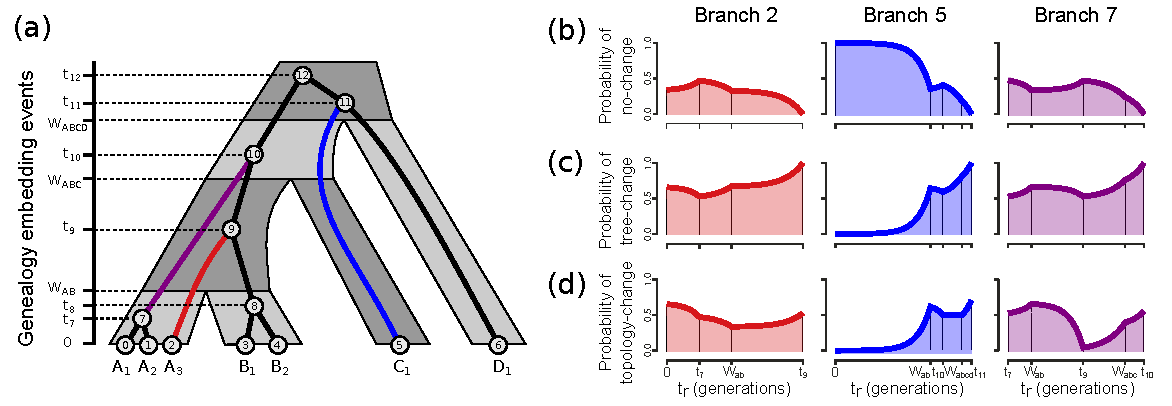
\includegraphics[width=0.99\textwidth]{figures/Fig1-embedding-and-probs-fill.pdf}
	\caption{
		The effect of recombination on a genealogy embedded in a species tree
		can be modeled using the MS-SMC'. 
		% A genealogy embedded in a species tree exhibits different probabilities
		% of outcomes of recombination, when viewed backwards in time, depending on 
		% the timing and branch on which recombination occurs.
		(a) A parameterized MSC model is composed of discrete intervals separated 
		by population divergence events ($W$), where the rate of coalescence can vary
		among intervals with different effective population sizes. The expected waiting
		time between coalescence events (e.g., $t_9$--$t_{10}$) is a product of these
		rates and the number of samples present, such that a table can be constructed of
		discrete intervals with constant rates (see Table 1). 
		% varies with respect to
		% changing rates of coalescence, as well the number of samples present at any time.
		% such that the an 
		 % and estimating
		% the expected waiting time between coalescence events (e.g., $t_9$--$t_{10}$) 
		% requires integrating over these rates as they change through time/intervals.
		% See Table 1 for the full genealogy embedding table for this 
		% and the number of samples changes.
		% by the rate of coalescence and the number of samples present.
		% reduce the number of samples present in an interval, whereas population 
		% divergence events (e.g., $W_{AB}$) increase the number in the subsequent interval.
		A recombination event occurring on a branch of a genealogy can cause
		three possible outcomes (b-d): "no change", "tree change", or "topology 
		change", and each branch exhibits piecewise variation in these 
		probabilities across discrete intervals. We derive solutions for 
		the relative probabilities of these outcomes in the main text by 
		integrating over the lengths of each branch in a genealogy. 
		Probabilities were calculated here for three selected branches as a 
		function of the time at which recombination occurs ($t_r$), given the 
		parameters in Table~S2 applied to the MSC model in (a).
	% 	divergence times ($W$) define ancestral populations. The population 
	% structure constrains which lineages of the genealogy can coalesce. Further, each 
	% population which can have a different effective population size ($N_b$),
	% which determine rates of coalescence within that population. Viewed backwards in time, 
	% coalescent events (e.g., $t_7$) in the genealogy reduce the number of samples, whereas 
	% species tree divergence events (e.g., $W_{AB}$) increase the number of samples present. 
	% (b-d) 
	% Recombination is modeled by detaching a branch at a specific time and 
	% sampling a waiting time until it re-coalesces, leading to either no change, 
	% a tree change (edge lengths), or topology change. We arbitrarily selected edges 2, 5, and 
	% 7 to illustrate how piecewise variation in coalescent rates back in time through the 
	% species tree leads to changing probabilities of each
	% outcome (discussed in Demonstration). Note that the values in (b) and (c) must sum to 1, 
	% since one of those two events must happen, while (d) is showing the probabilities of a 
	% subset of the events in (c). See Table 1 for the full genealogy embedding table for this 
	% example.
	}
	\label{fig:fig1}
\end{figure}


Importantly, both the coalescent and MSC are models of the expected distribution of 
\emph{unlinked} (uncorrelated) genealogies.
%(non-autocorrelated) genealogies. % sampled from throughout the genome. 
By contrast, two linked genealogies that are drawn from nearby regions of a genome %the genome 
are expected to be more similar than two random draws under these models. This spatial 
autocorrelation is a consequence of shared ancestry among samples at nearby regions, 
which decays over time and distance as recombination events reduce their shared ancestry.
This process can be approximated by randomly detaching an edge on a genealogy and sampling
a waiting time (based on the lineage effective population size) until it reconnects
to the genealogy at a different shared ancestor (Fig.~\ref{fig:figS-recomb-types}). 
In this way, the coalescent with recombination 
can be viewed as a process 
where a set of samples at the present substitutes one ancestor for another on 
either side of a recombination breakpoint. 
% \citep{wiuf_recombination_1999}. 
As a data structure, the spatial pattern of linked genealogies spanning
intervals between recombination breakpoints can be represented either as an 
ancestral recombination graph (ARG)
\citep{griffiths_ancestral_1996} or tree-sequence \citep{kelleher2016efficient}
(hereafter we will refer to it generically as an ARG; Fig.~\ref{fig:fig2}).

An algorithm to simulate the coalescent with recombination was developed 
early on 
% shortly after the coalescent
\citep{hudson1983properties}
% , however only with recent advances has it become 
% tractable to scale such simulations to larger, genome-wide scales 
% \citep{kelleher2016efficient}. 
% former new paragraph
% Although it is relatively simple to simulate the coalescent with recombination it has
% proven more challenging to develop an analytical solution for its expected outcome. 
%however it has proven challenging to develop analytical solutions for expected outcomes. 
%This includes 
% the a inference of 
%coalescent times on 
as a method for stochastically generating ARGs.
% yielding 
% a distribution of linked genealogies associated with intervals
% between recombination breakpoints across a genome.
% and the
% as well as the 
% distribution of 
% brakpoints across the genome where recombination occurred.
% (i.e., "waiting distances").
 % between genealogies).
Implicit to this process is an assumption that recombination 
occurs at some predictable rate from which the expected waiting 
distance between recombination events can be modeled as an exponentially 
distributed random variable. 
% (we will refer to ARGs hereafter; Fig. S1).
% While our ability to simulate the coalescent with recombination has made substantial progress, likelihood-based inference of recombination events and coalescent times (that is, the ancestral recombination graph -- "ARG") is notoriously difficult \citep{griffiths_ancestral_1996}. 
% Unfortunately, although 
Although generating ARGs consistent with a demographic model is 
relatively simple, inferring an ARG from sequence data -- composing  
recombination breakpoints and local genealogy inferences -- remains highly 
challenging. This stems in part from the great complexity of this problem, 
% and the challenge of distinguishing among many equally probable 
% results given limited information between recombination events;
but also reflect limitations of our current models for 
extracting historical information from linked genome data.

% about linked genealogies.
% infinite series of genealogies can often yield similar
% likelihoods 
% inferring ARGs from sequence data remains challenging, as it is
% computationally intensive, and can be nearly infinite in 
% possibilities for large genome lengths and numbers of samples.
% This stems from the relatively small amount of information 
% This stems mostly from the 
% in part from a relative dearth of models for 
% predicting the similarity of genealogies across different 
% genomic distances.
% or expected
% patterns of genetic linkage across large genomic distances.
% modeling expectations for patterns of genetic linkage across 
% different genomic distances in ARGs remains challenging. 
% linked information in ARGs remains challenging, which in turn limits the 
% amount of information that can be extracted from sequence data for ARG inference. 
% This in turn limits the amount of information that can be extracted from
% sequence data for 
% The problem of inferring ARGs is thus
% computationally intensive, and can be nearly 
% infinite in possibilities for large 
% genome lengths and numbers of samples \citep{mcvean2005approximating}. 
% to perform poorly. 
% have difficulty distinguishing among a nearly infinite range 
% of equally probable results using the limited amount of information 
% present between recombination events. 
% Consequently,
% inferring an ARG from sequence data 
% However, inference of ARGs 
% remains highly challenging, as it 
% is computationally intensive, highly limited by 
% sequence information, and can be nearly infinite in possibilities for large 
% genome lengths and numbers of samples \citep{mcvean2005approximating}. 
% In other words, there
% are usually very few mutations to provide information about each genealogy, 
% and ...
A major advance was achieved through development of the Sequentially Markov 
Coalescent (SMC), a simpler approximation of the coalescent with recombination
that restricts the types of recombination events that can occur. Specifically,
an edge that is detached from a genealogy by recombination is allowed only to
re-coalesce with ancestral lineages that contributed genetic material to samples
in that interval (as opposed to re-coalescing with any ancestral lineage). 
% the types of coalescent events that can occur between sequential
% space of possible ARGs that 
This greatly reduces the space of possible ARGs without changing the expected
distribution of sequential genealogies, and in doing so enables modeling
changes between sequential genealogies
% This restricts the types of coalescent events that can occur between 
% sequential genealogies, in a way that enables modeling 
% changes between
% models 
% changes among sequential genealogies 
% them 
as a Markov process 
\citep{mcvean2005approximating}. 
% Implicit to SMC-based methods is the expectation that recombination occurs at 
% some rate from which the waiting distance between recombination events can be modeled 
% as an exponentially distributed random variable. 
Under these assumptions a tractable likelihood framework can be developed. 
% inferring modeling
% The SMC provides a generative framework for producing a set of genealogies
% and segment lengths under a set of rules 
% The SMC (and related methods) provides a likelihood function 
% for the probability of observing a sequence of genealogies 
% pairwise coalescence times 
% and corresponding segment lengths between them on a genome, 
% given an effective population size and recombination rate. 
% 
% provides a generative framework for genealogies and segment lenghts under 
% a set of rules on which likelihood inference methods can be developed...
% 
% NEXT< start with Because, or something, not however,... 'this is how it is implemented in hmms'
% However, 
Because neither genealogies or segment lengths can
be observed directly, most SMC-based inference methods use 
% employ 
hidden Markov model (HMM) methods that treat these as hidden states 
which influence observable changes in sequence data.
% be inferred from sequence data. 
% he segment lengths and coalescent times are unknown, most methods use hidden Markov 
% model (HMM) methods in which these are hidden states inferred from sequence 
% data. 
% Further extensions have been developed for modeling variable 
Examples of inference tools built on the SMC framework include 
PSMC \citep{li2011inference} and MSMC \citep{schiffels_inferring_2014}
which use pairwise coalescent times between sequential genealogies
to infer changes in effective population sizes through time, 
and ARGweaver \citep{rasmussen2014genome, hubisz2020inference}, 
which infers ARGs from genome alignments using an SMC-based 
conditional sampling method.
% for inferring changes in effective population sizes
% of single or multiple populations through time, respectively, 
% based on pairwise coalescent times between sequential genealogies;
% % tools for inferring changes in effective population 
% % sizes through time of single (PSMC) or multiple populations (MSMC) 
% % based on pairwise coalescent times \citep{li2011inference, schiffels_inferring_2014}, 
% % , which methods for inferring ARGs using SMC-based conditional 
% % sampling methods
% % based on SMC-like simulations
% %\citep[ARGweaver;][]{rasmussen2014genome, hubisz2020inference}.
% and ARGweaver \citep{rasmussen2014genome, hubisz2020inference}, 
% which infers ARGs from genome alignments using an SMC-based 
% conditional sampling method.

% –- using an approach similar to 
% algorithms for simulating the coalescent with recombination –- 

% However, by modeling the coalescent with recombination
% using a Markovian approximation called the Sequentially Markov Coalescent (SMC), ARG 
% inference becomes more tractable.   
% The SMC is a simplification of the space of possible ARGs -- using an approach similar 
% to the algorithms for simulating the coalescent with recombination -- that models changes
% among sequential genealogies as a Markov process \citep{mcvean2005approximating}.
% IS THIS TECHNICALLY CORRECT?
% \hl{Under the SMC, the likelihood of a sequential set of genealogies and recombination 
% breakpoints (i.e., an ARG) is computed as the product of the set of independent likelihoods
% of observing each change from one genealogy to the next, given an effective population size
% and recombination rate.}
% While explicit likelihood-based inference of ARGs is still difficult, the SMC has enabled 
% \hl{several heuristic approaches to estimating ARGs from sequence data based on inferred 
% recombination events and differences in coalescent times among linked genealogies}
% \citep{li2011inference,rasmussen2014genome,hubisz2020inference}.
% , and the similarities among sequential genealogies, to model
% changes in effective population sizes \citep{}, and to infer 
% ARGs from sequence data 
% historical inferences about changes in effective population sizes, 
% recombination rates, and selection 


% Is this paragraph important? Maybe move to discussion. Concatalescence is not super important to intro.
% Despite the many advances that have been developed for incorporating information 
% from recombination into coalescent inference, the MSC framework (and related 
% fields in phylogenetics, such as the network multispecies coalescent 
% \citep{degnan2018modeling}) continues to largely treat recombination as a source 
% of error as opposed to information.
% This stems from the widely known expectation that, in parts of parameter space, 
% concatenation of sequences from multiple distinct genealogical histories can mislead
% phylogenetic inference. If a concatenated sequence is used to infer a single tree
% representing the species relationships, it might converge on a topology that is different
% from the species tree topology \citep{degnan2006discordance,kubatko2007inconsistency}. 
% The same concatenation biases can affect the distribution of inferred gene trees at
% individual loci as well, with potential effects on species tree or network inference
% methods that take multiple gene trees as inputs -- a process termed "concatalescence"
% \citep{gatesy_concatenation_2013}. The extent to which genetic loci (e.g., exons, UCEs,
% genome windows) represent a single versus multiple genealogical histories can be 
% estimated with coalescent simulations under an MSC model with recombination 
% \citep{mckenzie2020multispecies}. However, analytical solutions have not been
% developed to describe these as distributions within a statistical phylogenetic framework. 


\begin{figure}[t]
	\centering
	%\fbox{\rule[-.5cm]{4cm}{4cm} \rule[-.5cm]{4cm}{0cm}}
	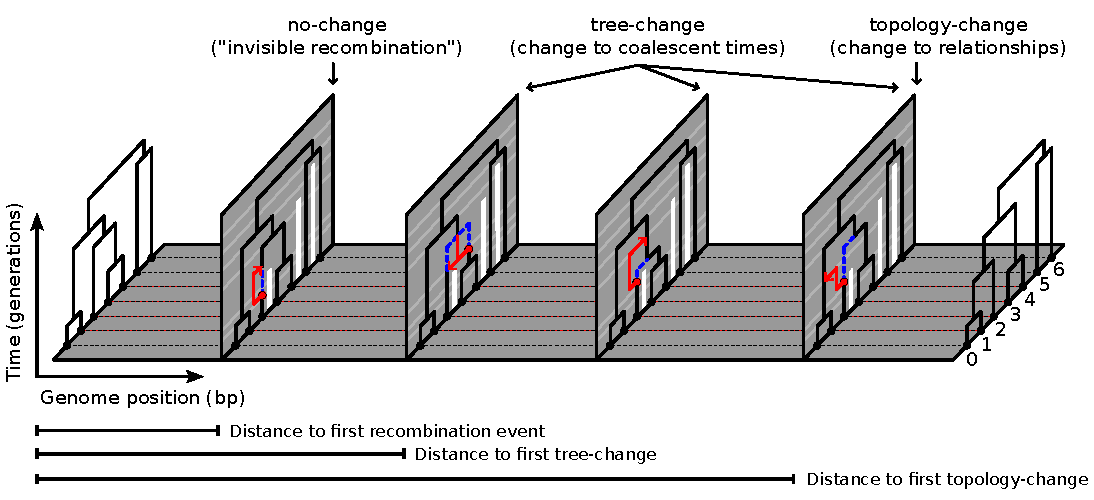
\includegraphics[width=0.99\textwidth]{figures/Fig2-ARG-recomb-types.pdf}
	\caption{
		% An ancestral recombination graph (ARG) with a demonstration of the coalescent
		% with recombination.
		% The MS-SMC' process demonstrated in an ancestral recombination graph (ARG).
		An ancestral recombination graph (ARG)
		is composed of a series of genealogies each spanning non-overlapping 
		intervals of a genome separated by recombination breakpoints. Here, 
		four recombination breakpoints separate the start and end positions 
		on a small chromosome in the history of a set of 7 samples constrained
		by a 4-tip species tree model (as in Figure 1).
		Recombination events are indicated as vertical panels, showing the process by 
		which a subtree (below the red circle) is detached and then re-coalesces (red arrow)
		with the remaining ancestral lineages. %, according to the MS-SMC' process. 
		The former edge (blue dotted) which existed throughout the interval to the left of a 
		panel is replaced by a new edge (red) through the subsequent interval. Vertical bars 
		(white) represent barriers to coalescence between samples in different species
		tree intervals (MSC model lineages).
		% ancestor is pruned (blue dotted) 
		% and replaced by a new sampled ancestor (red).
		Four categories of recombination events are shown from left to right, representing
		different outcomes based on the lineage with which a detached subtree re-coalesces:
		no-change; tree-change resulting in a shortened coalescence time; 
		tree-change resulting in a lengthened coalescence time; and tree-change 
		resulting in a different topology. These can be further consolidated into 
		three \emph{event types}: (1) no-change, (2) tree-change, and (3) topology-change.
		Every recombination event causes either a no-change or tree-change event, whereas
		a topology-change is a subset of possible tree-change events. The expected waiting
		distance until a specific recombination event type occurs can be calculated under 
		the MS-SMC' given a starting genealogy, MSC model, and %per-site per-generation 
		recombination rate.
	% Examples of the four different categories of outcomes from a 
	% recombination event (adapted from \citep{deng_distribution_2021}). 
	% (a) A category 1 event occurs when the dislocated lineage reattaches to the 
	% original lineage. 
	% (b) A category 2 event occurs when a dislocated lineage attaches to its 
	% sibling lineage (the lineage that it originally coalesced with), shortening 
	% both of their branch lengths and extending that of its parental lineage. 
	% (c) A category 3 event occurs when the dislocated lineage attaches to its 
	% parental lineage, lengthening the original lineage and its sibling lineage,
	% and shortening the parental lineage.
	% (d) A category 4 recombination event occurs when the dislocated lineage
	% attaches with any lineage other than itself, its sibling lineage, and its
	% parental lineage. This is the only category of recombination event that
	% changes the topology of the genealogy.
}
\label{fig:fig2}
\end{figure}


% Implicit to SMC-based methods is the expectation that recombination occurs at 
% some rate from which the waiting distance between recombination events can be modeled 
% as an exponentially distributed random variable. 
\cite{marjoram2006fast}
described an important extension to the SMC, termed the SMC', for additionally
modeling "invisible" recombination events, where a detached lineage re-attaches
with its own ancestral lineage prior to the time of its next coalescent event. 
This leads to no change in the genealogies between two sequential intervals, 
despite the occurrence of a recombination between them. The inclusion of
such events has been shown to 
% , such that 
% no change between 
% neighboring genealogies, which has been shown to 
significantly improve SMC-based inference methods \citep{wilton2015smc}. 
Under the SMC', a detached lineage can thus re-coalesce with an allowable 
ancestral lineage over a continuous range of time, leading to one of 
four possible categorical patterns for the relationship between two
sequential genealogies
% a change 
% relative to the previous genealogy that can be described as one of 
% \hl{four possible categorical} outcomes:
% of possible outcomes of recombination, 
(Fig.~\ref{fig:fig2}, Fig.~\ref{fig:figS-recomb-types}): 
(1) no change %between sequential genealogies;
(2) shortening of a coalescent time; (3) lengthening of a coalescent time; 
and (4) %a coalescent event that changes the topology (relationships). 
a change to the genealogical topology (relationships).
These can be grouped more generally into \hl{three types}: 
"no-change" (category 1), "tree-change" (categories 2-4), and "topology-change"
(category 4). Recently, \citet{deng_distribution_2021} derived a set of solutions for
the expected waiting distances to each of these three types of 
outcomes for a single population with constant effective population size.
% Although all three outcomes, and their associated waiting distances, occur 
% implicitly between sequential genealogies within data generated under the SMC', 
% there was not previously a solution for expectations between events that do 
% not occur sequentially, representing the joint probabilities of multiple events.
% This provides an important advance, for establishing a neutral expectation for 
% turnover 
% in different categorical types of genealogy changes, and for connecting these
% to coalescent model parameters, which may prove useful for future ARG inference 
% tools. 
This provides an important advance by establishing a neutral expectation 
not only for the distance until any generic recombination event occurs, 
but more specifically, for % the different expectations for 
% for 
different types 
of events that leave different detectable signatures in the genome.
% not
% only for any generic recombination events to occur, but for different types 
% of events that leave different detectable signatures in the genome.
% ,which may prove useful for the development of future SMC'-based tools.
% in genealogical topologies, and for connecting coalescent model parameters to these
% outcomes, which may prove useful for future advances in ARG inference. 

% \citep{deng_distribution_2021} recently 
% Their solution assumes a single population with constant effective population size, 
% but nevertheless ... 
% Their solutions 


% recently described a partitioning of different possible outcomes of recombination 
% events into three categories: (1) "no effect", which do not change the genealogy; 
% (2) "tree changes", which affect only coalescent times (edge lengths); and 
% (3) "topology changes", which affect the genealogical relationships.

% the expected waiting distances between
% recombination events, describing different rates for three categorical
% types of recombination events that can occur (Fig.~\ref{fig:fig2}). 
% % 
% This includes recombination events that: (1) have no affect on the 
% genealogical tree; (2) cause "tree changes" (i.e. that they 
% affect either the branch lengths or the topology of the genealogical tree, 
% as in any of categories 2, 3, and 4), and those that cause "topology changes" 
% (only category 4) (\textbf{Figure 1}).


% \citet{deng_distribution_2021} derived an approximate solution for the 
% distribution of waiting distances between sequential genealogies in an ARG. 
% This involved extending the simple expectation for the expected waiting distance
% between *any* recombination event, and partitioning the results into categories
% of different possible outcomes (Fig.~\ref{fig:fig2}). 

% , some of which result in changes to 
% the genealogy, and others of which do not. 
% This represents a major advance. Although 
% The expected waiting distance between any recombination event can be modeled as
% a simple simply described by an exponential distribution}, 
 % under the SMC’ 

% an extension of the SMC that includes "invisible" recombination
% events that result in no change between neighboring genealogical trees. 
% \hl{was known previously}, 
% \citet{deng_distribution_2021} 


Here, we extend the methods of \citet{deng_distribution_2021} to an MSC framework
to approximate the expected waiting distances between different types of 
genealogy changes under a parameterized species tree model. In this respect, 
the waiting distances between recombination events that cause topology-change 
may be of greatest interest, as they leave the most detectable signatures 
in sequence data, and are relevant to expected gene tree distributions that form
an important component of many MSC-based methods.
The waiting distance until a topology-change event can include multiple
intervening recombination events of the no-change or tree-change type
(Fig.~\ref{fig:fig2}). 
The relative occurrence of events that do not result in topology 
changes can be especially high in small sample sizes \citep{wilton2015smc}, 
which are common in MSC-type datasets, since samples are partitioned 
among species tree intervals. 
% The partitioning of 
% recombination events that of categories 1-3 occur 
% disproportionately often in small sample sizes \citep{wilton2015smc}, 
% which are especially common in MSC-type datasets since
% samples are partitioned among species tree intervals. 
The partitioning of 
coalescent events among species tree intervals is thus expected to constrain 
the types of recombination events that will be observed. Consequently, the
distributions of waiting distances between different types of 
genealogy changes should be highly dependent on, and thus informative about, 
the species tree model. We refer to this general framework of embedding the 
SMC' in an MSC model as the MS-SMC'.


% The relative frequency
% of different event types is therefore expected to be contingent on parameters
% of the species tree. 

% Recombination events of type 4 are of greatest interest
% % the most inherently interesting 
% for most applications,
% % because s
% as they leave the most detectable signal in sequence data.
% % since they will produce the most obvious signal in the sequence data. 
% However, events of types 1-3 occur disproportionately often in small sample 
% sizes \citep{wilton2015smc}, which are especially common in MSC-based studies, 
% where genealogies are embedded within a species tree, such that fewer samples 
% typically represent each lineage. But the
% relative frequency of the different events is contingent upon the Ne values of the
% species tree branches and on the species divergence times. In other words, the 
% partitioning of coalescence events among lineages of the species tree topology is
% expected to constrain the types of recombination events that are more likely to be
% observed. This results in distributions of waiting distances between genealogical
% changes being highly dependent upon parameters of the species tree model. 

% With this in mind, we extend the method of \citet{deng_distribution_2021} to the MSC
% to predict the expected waiting distances between genealogy changes under a 
% parameterized species tree model. This new solution is important for establishing an 
% expectation for the neutral rate of genealogy turnover under different species tree 
% parameterizations. It may also have applications for ARG inference under complex 
% demographic models \citep[e.g.,][]{hubisz2020mapping}, potentially serving as a 
% component of a likelihood function for inferring species trees from linked 
% genealogies -- a future theoretical goal.

% MS-SMC: multispecies sequentially markovian coalescent
% SM-MSC: sequentially markovian multispecies coalescent

%Solutions exist for simulating genomes under the coalescent with recombination \citet{ipcoal, kelleher, hudson}. In particular, \emph{msprime} is a powerful and flexible tool for simulating ancestral recombination graphs for many samples under user-defined demographic scenarios. \emph{ipcoal} is an extension of msprime that accepts multispecies coalescent parameters. 

%Phylogenetic methods sampling regions throughout the genome have increasingly adopted the multispecies coalescent model to incorporate variation in regions due to incomplete lineage sorting. Applications of the multispecies coalescent in phylogenetic inference aim to avoid known bias under which, in certain circumstances, phylogenies inferred from concatenated data might converge on a tree that is not the species tree. One challenge of applying the multispecies coalescent for species tree inference is properly defining the breakpoints for loci used in the analysis. Often this is done arbitrarily: researchers ensure that loci are long enough to infer reliable gene trees, and that there are enough inferred gene trees to infer a robust species tree. However, there has been some debate in the literature over the effects of locus length on species tree inference. Specifically,  

%Another way in which the ancestral recombination graph is relevant to phylogeneticists is for local inference...

%Recently, \citet{deng_distribution_2021} provided a solution for the distribution of waiting times to genealogical changes under the SMC', a popular model for simulating ancestral recombination graphs. However, their solution is constrained to a single population of constant effective population size.

%Establishing the predicted length of different topologies along the chromosome is important for inference of local genealogies in population genetics, which can be used for inference of selection, demographic changes, and introgression. It is also important in multispecies coalescent methods in phylogenetics, which often rely on inference of gene trees.


% springer + gatesy

% inference, argweaver-D

\section{Approach}
\subsection{Comparison to \citet{deng_distribution_2021}}

Our approach is a generalization of the \citet{deng_distribution_2021} derivation 
of waiting distances to genealogy changes for a single population of constant size. 
We modified the single-population model to (1) include barriers to coalescence imposed
by a species tree topology, and (2) integrate over changing coalescence rates along
paths through multiple species tree intervals with different effective population 
sizes. 
% I don't feel particularly inclined to follow their variables. I think it would be
% cleaner to translate it to cleaner variables to align better with MSC theory.
We have intentionally reproduced our equations in a similar structure and using
many of the same variable names as in \citet{deng_distribution_2021}.
% to highlight the changes we made to generalize their solution.


\subsection{MSC model description}
% We assume a species tree model with divergence times in units of generations and 
Given an MSC model composed of a species tree topology ($\mathcal{S}$), with divergence
times ($W$) in units of generations, and constant \hl{diploid} effective population sizes
assigned to each branch ($N_b$), a genealogy ($\mathcal{G}$) 
for any number of sampled gene copies can be generated by randomly sampling 
coalescent times %($t$) 
at which to join two samples into a common ancestor, 
starting from samples at the present in each interval. The rate of coalescence
is $\frac{1}{2N_b}$, and the expected waiting time between coalescence events
that will reduce the number of samples from $k$ to $k$-1 in a population 
follows the Kingman coalescent:

\begin{equation}
	\mathbb{E}(t_k| N) = \frac{k(k-1)}{2N}
\end{equation}

\noindent In a single population model
with constant $N$ this rate decreases monotonically as the number of remaining 
samples after each coalescence event decreases. In an MSC model, however, 
the rate of coalescence typically waxes and wanes through time, as the
transition from one branch interval to the next can be associated with 
different N$_b$ and an increase in $k$ as samples from 
descendant branch intervals are merged.

Based on this generative framework for sampling genealogies, a set of likelihood
solutions have been developed to fit coalescent model parameters, such as 
$N$ in single population models \citep{kingman1982coalescent},
or $N_b$ and $W$ in MSC 
models \citep{rannala2003bayes}, based on inferred coalescent times. 
In the latter framework, each species tree branch interval is treated independently, 
such that the likelihood of a genealogy embedding is calculated from the joint
probability of observing each distribution of coalescent waiting times within
each species tree branch interval. A key feature of these equations is that 
when $k$ lineages are present, we can use equation 1 as a rate parameter ($\lambda$)
to calculate the likelihood of an observed coalescent waiting time ($t_k$) between
$k$ and $k$-1 lineages from an exponential probability density:
% for the expected rate
% of coalescence
% between when $k$ and $k$ - 1 lineages exist. 
%  and thus the probability of 
% when Using the expected time between coalescence
% events when $k$ lineages are present (equation 1) as a rate parameter, the 
% likelihood of an observed waiting time can be calculated from an exponential 
% probability density. 
	
\begin{equation}
	% \mathcal{P}(t_k|\lambda) = \lambda e^{-\lambda t_k} 
	f(t_k) = \lambda e^{-\lambda t_k} 	
\end{equation}


% In each species tree interval this is repeated for each interval between 
% observed coalescent events.

% The probability of a particular genealogical topology among a set of coalesced
% samples in an interval. The probability a particular pair of lineages coalesce
% is 1 ( kchoose2) = (2 / (j * (j - 1))), where j=m, n, n+1. [Describe m and n as
% the start and end of intervals.]

% \begin{equation}
% 	\mathbb{P}(t_k | N_e) = 
% 		\frac{1}{2N_e} 
% 		\exp \bigg\{-\frac{k(k-1)}{4N_e} t_k \bigg\} \times 
% 		\exp \bigg\{-\frac{n(n-1)}{4N_e} (\tau - (t_m + t_{m-1} + \text{...} + t_{m+1})) \bigg\}
% \end{equation}

% Similarly, the likelihood of observing a set of coalescent
% times on a genealogy embedded in a species tree can be calculated from the
% joint probability of its observed coalescence times within each interval
% \citep{rannala2003bayes}, treating intervals independently. 
% Thus, the genealogy (G) in Figure 1 can be calculated as
% ...

% Generating unlinked genealogical trees under the MSC is straightforward: Coalescent events between samples can only happen after (moving backward in time) coalescence of the species that contain them, and the coalescent rate in each part of the tree is dependent on both the number of genealogical lineages that can coalesce in that section and on the effective population size in that section.

\subsection{MS-SMC' model description and notation}

% Under the single-population SMC' 
% considered by \citet{deng_distribution_2021}, the 
Under the SMC' model, sampling of a linked genealogy requires considering not only 
%a species tree and its parameters, 
coalescent model parameters, 
as we did above, but also an existing genealogy -- it is a method 
for sampling the next genealogy conditional on the previously observed one. 
If we define the previous genealogy as $\mathcal{G}$, and the sum of its edge lengths 
as $L(\mathcal{G})$, then under the assumption of a constant recombination rate through time,
a recombination break point can be uniformly sampled from $L(\mathcal{G})$ to occur with 
equal probability anywhere on $\mathcal{G}$. 
% on any branch.
A recombination event creates 
a bisection on a branch, separating a subtree below the cut 
from the rest of the genealogy (Fig.~\ref{fig:fig2}). 
The subtree must then be reconnected by sampling a new common 
ancestor between it and the other samples still connected to the genealogy, which 
must occur above the time of the cut. This re-connection point is sampled 
probabilistically with an expected waiting time until re-coalescence the 
same as described above (equations 1 and 2).

In a single population model with constant $N$ the re-coalescent probability
after a recombination event decreases monotonically, as each subsequent 
coalescence event decreases $k$.
% (e.g., Fig.~1B). 
Once again, the MSC model 
differs from this: coalescent events similarly decrease $k$, but the merging of 
species tree branches into ancestral intervals increases $k$, and effective population 
sizes can also vary among species tree intervals. 
Thus, the probability that a subtree re-connects to the genealogy can vary 
along its path of possible reconnection points through 
different species tree intervals
(Fig.~\ref{fig:fig1}b-d). 
A species tree can thus be decomposed into a series of relevant intervals 
between events that change the rate of coalescence,
% , including within species tree intervals, 
which we refer to as the genealogy embedding table (Table~\ref{tab:table-1}). 
From this table it is possible to calculate the probabilities of different
recombination event type outcomes, and consequently, to model the expected 
waiting distances until specific recombination event types occur. 

% Using this information on the rate of coalescence within each genealogy
% embedding interval, it is then possible to model the probability that a
% detached lineage will re-coalesce within any specific interval. From this, 
% it is then possible to calculate probabilities of different recombination event types which 
% are a
% Our goal ... The goal of the MS... To model the probabilities of different
% genealogy change events we must model the probability that a detached lineage
% will re-coalesce with any allowed ancestral lineage while constrained by the
% MSC model. This requires integrating over the coalescence rates which can 
% vary among intervals of the species tree model.

To better understand the relationship between the MS-SMC' and the genealogy
embedding table, consider a specific branch ($b$) from Fig.~\ref{fig:fig1}. 
Branch 7 on the genealogy spans four relevant intervals, 
labeled as rows 1, 6, 7, and 8 in Table~\ref{tab:table-1}.
The coalescent rate within each interval can be calculated from its
\hl{diploid} effective population size ($n_i$) and number of samples 
present ($a_i$). The time at the start of each interval is $\sigma_i$. 
We define an additional variable, $\mathcal{I}_b$, to represent the 
number of intervals spanned by a branch, such that, for example, 
$\mathcal{I}_7$=4. 
% This is used in the equations below as an
% index to iterate over the ordered sequence of intervals on a branch. 
By iterating over all $i$ intervals from 0 to $\mathcal{I}_b - 1$ 
different rates can be applied to different intervals over the length 
of a branch.
% (this can be found by searching for the branch label in the \emph{branches} 
% column of the table). 
% We record the number 
% of intervals in which a branch is present as $\mathcal{I}_b$, such that,
% for example, $\mathcal{I}_7$=4. We use this indexing variable to iterate
% over the ordered sequence of intervals on a branch. 
% over the lengths of each interval on a branch. 
% The coalescent rate within each genealogy embedding interval of the
% table is calculated from the \hl{diploid} effective population size ($n_i$) 
% and number of samples present ($a_i$).
% to the end of the last interval $\sigma_{\mathcal{I}_{b+1}}$.
% For this branch, we are interested in defining intervals where 
% coalescent rate parameters change, 
% which involves identifying coalescent events that occur in the same species
% tree intervals as this branch, as well as events where this branch 
% transitions from one species tree interval to the next.
% To do so, we must identify times at which there are relevant coalescent events 
% between other lineages in the same population, or at which there are relevant 
% species merging events. 
% This involves examining the genealogical tree as it is 
% embedded within the species tree. With the genealogy embedding table, we can 
% In the genealogy embedding table we can then query the "branch" column to
% isolate intervals involving branch 7. This corresponds to rows 1, 6, 7, and 8, 
% such that the number of intervals on branch 7 ($\mathcal{I}_b$) is four. 
% The time of the start of each interval ($i$) is $\sigma_i$. 
% \hl{An integer index ($\mathcal{I}$) stores the number of intervals that 
% each branch occurs in, such that enumerating over the range
% of $\mathcal{I}_b$ visits each interval in order along 
% genealogy branch $b$.} 
% easily isolate the intervals specific to edge 7 by querying the "branches" 
% column of the table and extracting the rows where this column contains our 
% focal edge (for edge 7, these are rows 1, 6, 7, and 8). 
% The number of rows is equal to the 
% The number of rows 
% we extract (in this case, 4) is equal to the number of intervals in the edge 
% ($\mathcal{I}_b$). If we retain the relative order of the rows and re-index them from 
% $0$ to $\mathcal{I}_b-1$, the information in the columns (e.g. $n_i$, $a_i$) is easily
% adapted for use in the equations presented below. 
% Each branch of $\mathcal{G}$ spans one or more intervals
% from which a lower and upper (min, max) bound for that branch can also be 
The upper and lower bounds of a branch are also recorded as 
$t_b^l$ and $t_b^u$, respectively. 
% extracted ($t_b^l$ and $t_b^u$, respectively). 
Later, we describe equations that require information about
how genealogy branches are related (e.g., parent-child or siblings), 
which can also be extracted from $\mathcal{G}$ and 
represented in a separate table (e.g., Table~S1).
% . For example, 
% edge 2 from Fig.~\ref{fig:fig1} and Table~\ref{tab:table-1} overlaps with 
% three intervals, such that $\mathcal{I}_2$ = 3.
% \hl{From this gene tree embedding we also define 
% the set $\mathcal{I}$ that includes the indices of all intervals in the table. 
% And we define an indexing variable $I_b$ for each branch ($b$) in $\mathcal{G}$ that
% returns a vector of ordered intervals ($i \in \mathcal{I}$) that overlap with 
% a specific gene tree branch.}
% For example, edge 2 from Fig.~\ref{fig:fig1} and Table~\ref{tab:table-1} overlaps with 
% three intervals, such that $I_2$ = (0, 1, 6). 
These variables, and the genealogy embedding table, 
together include all relevant parameters for the derivations below. 



% To summarize, the genealogy embedding table is simply a set containing all 
% unique intervals (and their properties) over all edges in the genealogy, 
% and it maps those intervals to the genealogy edges to which they belong. 
% This allows us to easily query relevant intervals for any edge of the 
% genealogical tree. For extracting relationships among branches (e.g. parent,
% sibling, as required for the topology cahnge equations), we can reference a 
% separate table specific to the structure of the genealogical tree only (see 
% Appendix, Table 2).
% , and are also summarized in the Appendix.

%\hl{needs updates to figure out how table can align with existing variables names.
%Additional table with final info could be supplement. Includes I, sister index, parent index...}

% Unlike in the single-population SMC', the intervals in the multispecies model
% are branch-specific. For example, the breakpoint $\sigma_{D1}$ in Figure 2c  
% corresponds to the species tree coalescence of species C and species D. This 
% increases the number of lineages available for the D lineage to coalesce with 
% (from 1 -- itself -- to 2) and might also change the effective population size.
% However, this breakpoint does not appear in Figure 2d since the lineage in species
% E is not able to coalesce with lineages from species C or D until $\sigma_{E1}$,
% when E coalesces with the ancestor of C and D in the species tree.


\begin{table}[h]
\centering
\caption{
	A genealogy embedding table for MS-SMC' calculations for the genealogy and
 	species tree in Figure 1. The rate of coalescence within each interval can 
 	be calculated from $a$ and $n$, and its length from $d$.
	% present ($k$) and the effective population size ($N_e$). 
	To integrate over the probability of coalescence on a specific genealogy
	branch (e.g., branch 7 from Figure~\ref{fig:fig1}) involves 
	integrating over all intervals that include that branch (e.g., rows 
	1, 6, 7, and 8).
}
\begin{tabular}[t]{ |c|c|c|c|c|c|c|c|c| }
	\toprule
	 % & start ($t_i^l$)  & end ($t_i^u$) 
	 & start ($\sigma$)  & end  & pop & $N$ ($n$)  & N edges ($a$) & coal  & length ($d$) & branches \\
	\midrule
	0 & 0          & $t_7$      & A   & $N_A$     & 3 & $t_7$    & $t_7$ - 0            & 0,1,2 \\
	1 & $t_7$      & $W_{AB}$   & A   & $N_A$     & 2 & -        & $W_{AB}$ - $t_7$     & 2,7   \\	
	2 & 0          & $t_8$      & B   & $N_B$     & 2 & $t_8$    & $t_8$ - 0            & 3,4   \\ 
	3 & $t_8$      & $W_{AB}$   & B   & $N_B$     & 1 & -        & $W_{AB}$ - $t_8$     & 8     \\
	4 & 0          & $W_{ABC}$  & C   & $N_C$     & 1 & -        & $W_{ABC}$            & 5     \\
	5 & 0          & $W_{ABCD}$ & D   & $N_D$     & 1 & -        & $W_{ABCD}$           & 6     \\
	% 
	6 & $W_{AB}$   & $t_9$      & AB  & $N_{AB}$  & 3 & $t_9$    & $t_9$ - $W_{AB}$     & 2,7,8 \\
	7 & $t_9$      & $W_{ABC}$  & AB  & $N_{AB}$  & 2 & -        & $W_{ABC}$ - $t_9$    & 7,9   \\
	% 
	8 & $W_{ABC}$  & $t_{10}$   & ABC & $N_{ABC}$ & 3 & $t_{10}$ & $t_{10}$ - $W_{ABC}$ & 5,7,9  \\
	9 & $t_{10}$   & $W_{ABCD}$ & ABC & $N_{ABC}$ & 2 & -        & $W_{ABCD}$ - $t_{10}$ & 5,10 \\
	%
	10 & $W_{ABCD}$ & $t_{11}$  & ABCD & $N_{ABCD}$ & 3 & $t_{11}$ & $t_{11}$ - $W_{ABCD}$ & 5,6,10 \\
	11 & $t_{11}$  & $t_{12}$   & ABCD & $N_{ABCD}$ & 2 & $t_{12}$ & $t_{12}$ - $t_{11}$ & 10,11 \\
	12 & $t_{12}$  & -          & ABCD & $N_{ABCD}$ & 1 & -        & -                   & 12    \\	
	\bottomrule
\end{tabular}
\label{tab:table-1} 
\end{table}



% In the MS-SMC', we specify a model with piecewise-constant coalescence rates. 
% However, intervals under the MSC adaptation are bounded not just by coalescence
% events in the \emph{genealogy} tree (decreasing the number of available lineages for 
% coalescence), but also by relevant coalescences in the \emph{species} tree. Species 
% coalesence events increase the number of genealogical lineages available for 
% coalescence, and they also can correspond to changes in effective population 
% size (\textbf{Figure 2}). 

% Having described our model, we also adopt the following notation:

% \begin{itemize}
%   \item $\mathcal{I}_b$: index of an interval on genealogy branch $b$. A genealogy 
%   branch is split into discrete intervals corresponding to points along its length 
%   at which either the species tree interval changes, or the number of samples $k$ with
%   which it can coalesce changes.
%   \item $t^u_b$: the height, in generations, of the upper bound of genealogy branch $b$.
%   \item $t^l_b$: the height, in generations, of the lower bound of genealogy branch $b$.
%   \item $\mathcal{T}$: the genealogical tree
%   \item $\mathcal{S}$: the species tree
%   \item $\mathcal{N}$: the number of tips in the species tree
%   \item $L(\mathcal{T})$: the total genealogical tree length, in generations
%   \item All summations where the stopping value is less than the starting value are equal to zero.
% \end{itemize}

% Several values are indicated only on one branch at a time, and thus we do not include 
% an underscore to indicate which branch. These are:
% \begin{itemize}
%   \item $\sigma_i$: the length, in generations, of the lower bound of interval $i$ on branch $b$.
%   \item $n_i$: the effective population size of species tree interval index $i$.
%   \item $a_i$: the number of available lineages to coalesce with in the genealogy interval with index $i$.
%   \item $T_i$: the length, in generations, of species tree interval with index $i$.
% \end{itemize}


\subsection{Deriving probabilities of genealogy changes in the MS-SMC'}
A recombination event occurring on $\mathcal{G}$ can result 
in three types of outcomes (Fig.~\ref{fig:fig2}).
Of these, there is a zero-sum relationship between a no-change and 
tree-change event, such that one or the other must occur.
% one or the other must always occur.
% , resulting in either 
% no change to the genealogy, a change only to its branch lengths, 
% or a change to its topology. 
Therefore, as a first step towards describing probability statements 
for each of these event types, we focus first on deriving the 
probability of a no-change event, which is the simplest outcome.
Then, from the law of total probability, we also have a result for 
the probability of a tree-change event. 
% From this, we can then calculate the probability of a tree-change
% by the law of total probability. 
% Therefore, our first step in deriving probability statements for
% Our first step in deriving probability statements for
% these different outcomes is to calculate the probability of a no-change event. 
Finally, to calculate the probability of a topology-change event, 
we derive a statement for the probability of a specific subset of 
tree-change events where the detached lineage is restricted in which
ancestral lineages it can re-coalesce with. 
% we calculate the probability of topology-change as a subset of
% the probability of a tree-change, in which we restrict which branches the
% detached lineage can re-coalesce with.
% events. 

% probabilities 
% of events that 
% fall into the other categories.
% In category 1, there is no change to the genealogy. In categories 2 and 3 only
% a the branch lengths of the genealogical tree change while the topology remains
% the same. In category 4, the topology of the resulting tree is different from the 
% original tree. For simplicity, we will refer to changes that affect only branch
% lengths (categories 2-3) as those that change \emph{the tree}, and category 4 as 
% those that change \emph{the topology}.
% Our first steps are to calculate the probability of a recombination event in
% category 1, where the new genealogical tree is identical to the previous tree. The 
% law of total probability then allows us to use the inverse probability to calculate
% a waiting distance to a change that falls into any of categories 2, 3, or 4. 

\subsubsection{Probability that recombination at $t_r$ on branch $b$ does not change the tree:}
% \subsubsection{Probability that a recombination event at time $t$ on branch $b$ will not change the tree:}
% \hl{these sections needs waay more description. What does this all mean? The text here
% was only restating the section title. You need to build up to the more complex ones by 
% walking the readers through the more simple examples. I think this is super important
% to make this work understandable. Think of Rannala and Yang 2003.}
We begin by assuming knowledge of when and where recombination takes place, in terms 
of a recombination event bisecting branch $b$ at time $t_r$. %The variable $\sigma$ 
% The index $i$ refers to the genealogy embedding interval in which recombination occurs.
For no genealogy change to occur the detached branch must re-attach to its original 
lineage during the same interval in which it detached.
If it connects to any other existing lineages during this same interval, 
or coalesces in a later interval, this would lead to a change in either the 
tree or topology. A derivation of this equation can be found in the Appendix.
Here, $i$ is the interval index in which recombination occurs (at time $t_r$). 
The first two terms correspond to the probability of detaching from the interval 
at $t_r$ and re-coalescing to the same branch within the same interval (i.e., $ii$),
and not re-coalescing with any other lineages present during this interval. The
last term describes the probability of re-coalescing with the same branch in a later 
interval (i.e., $ij$), and not re-coalescing with any other samples present in any
later intervals on this same branch. 

% PREVIOUS APPROVED EQUATION 3
\begin{equation}
\begin{aligned}
	&\mathbb{P}(\text{no-change} | \mathcal{S},\mathcal{G},b,t_r) = 
	\frac{1}{a_i} + f(i,i) \exp \bigg\{\frac{a_i}{2n_i}t_r\bigg\} +
	\sum_{j=i+1}^{\mathcal{I}_b - 1} f(i,j) \exp\bigg\{\frac{a_i}{2n_i}t_r\bigg\} 
\end{aligned}
\end{equation}


\noindent This includes the following function which returns constant values 
representing the piece-wise constant probabilities of re-coalescence when
recombination occurs in interval $i$ and re-coalesces in interval $j$. This
function will reappear in later equations.

\begin{equation}
\begin{aligned}	
	f(i,j) = 
	\begin{dcases}
		- \frac{1}{a_i} \exp \bigg\{-\frac{a_i}{2n_i}\sigma_{i + 1} \bigg\}, 
		& \text{if } i=j\\
		% 
		\frac{1}{a_j} \left(1 - \exp \bigg\{ -\frac{a_j}{2n_j} d_j \bigg\} 
		\right)
		% \times
		\exp \bigg\{ -\frac{a_i}{2n_i}\sigma_{i+1} - 
		\sum_{q=i+1}^{j-1} \frac{a_q}{2n_q} d_q \bigg \}, 
		& \text{if } i\ne j\\
	\end{dcases}
\end{aligned}
\end{equation}

% PREVIOUS APPROVED EQUATION 4
% \begin{equation}
% \begin{aligned}
% 	% &P_{ii} = - \frac{1}{a_i} \exp \bigg\{-\frac{a_i}{n_i}(t_i^u - t_r) \bigg\} 
% 	&P_{ii} = - \frac{1}{a_i} \exp \bigg\{-\frac{a_i}{n_i}\sigma_{i + 1} \bigg\} 	
% \end{aligned}
% \end{equation}

% \begin{equation}
% \begin{aligned}
% 	&P_{ij} = 
% 	\left( \frac{1}{a_j} (1 - \exp \bigg\{ -\frac{a_j}{n_j} d_j \bigg\} \right)
% 	\times
% 	\exp \bigg\{ -\frac{a_i}{n_i}\sigma_{i+1} - 
% 	\sum_{q=i+1}^{j-1} \frac{a_q}{n_q} d_q \bigg \}
% \end{aligned}
% \end{equation}


% \begin{equation}
% \begin{aligned}
% 	&\mathbb{P}(\textrm{tree unchanged} | b,t,\mathcal{T},\mathcal{S}) = \frac{1}{a_i} +P_{ii}e^{\frac{a_i}{n_i}t}+ \sum_{k=i+1}^{\mathcal{I}_b-1} e^{\frac{a_i}{n_i}t} P_{ik}, \\
% 	&\text{where} \\
% 	&P_{ii} = - \frac{1}{a_i}e^{-\frac{a_i}{n_i}\sigma_{i+1}}, \\
% 	&\text{and} \\
% 	&P_{ik} = \exp\left(-\frac{a_i}{n_i}\sigma_{i+1}-\sum_{q=i+1}^{k-1} \frac{a_q}{n_q}T_q\right)\left(\frac{1}{a_{k}}(1-e^{-\frac{a_{k}}{n_{k}}T_{k}})\right),
% \end{aligned}
% \end{equation}

\subsubsection{Probability recombination on branch $b$ will not change the tree:}
By integrating the previous equation across all times at which recombination could
have occurred on branch $b$ (assuming a uniform recombination rate through time) 
we obtain the probability that recombination on this branch does not change the tree:

\begin{equation*}
	\mathbb{P}(\textrm{no-change} | \mathcal{S},\mathcal{G},b) = 
	\frac{1}{t^u_b-t^l_b} \int_{t_b^l}^{t_b^u} 
	\mathbb{P}(\textrm{no-change} | \mathcal{S},\mathcal{G},b,t)dt
\end{equation*}

\begin{equation}
	= \frac{1}{t^u_b - t^l_b}
	\sum_{i=0}^{\mathcal{I}_b-1} \frac{1}{a_i} d_i + 
	\frac{2n_i}{a_i} 
	\bigg(
		\exp\bigg\{\frac{a_i}{2n_i}\sigma_{i+1}\bigg\} - 
		\exp\bigg\{\frac{a_i}{2n_i}\sigma_i\bigg\}
	\bigg)
	\bigg(\sum_{j=i}^{\mathcal{I}_b-1}f(i,j)\bigg)
\end{equation}


\subsubsection{Probability that a recombination event will not change the tree:}
Finally, by summing across all branches on the tree 
% while assuming a uniform recombination rate through time and across branches, 
we get the probability that a recombination event occurring anywhere on 
$\mathcal{G}$ will result in a no-change event. %category 1 outcome.

\begin{equation}
	\mathbb{P}(\textrm{no-change} | \mathcal{S},\mathcal{G}) = 
	\sum_{b \in \mathcal{G}}
	\left[\frac{t^u_b - t^l_b}{L(\mathcal{G})}\right]
	\mathbb{P}(\textrm{no-change} | \mathcal{S},\mathcal{G},b)
\end{equation}

\subsubsection{Waiting distance to the next tree change:}
Under the SMC' the rate at which recombination events occur ($\lambda_r$)
is a product of the per-site per-generation recombination rate ($r$) and 
total branch lengths (in units of generations) of the current genealogy.

\begin{equation}
	\lambda_{r} = L(\mathcal{G}) \times r
\end{equation}

\noindent And thus a waiting distance ($x$) to the next recombination event 
spatially along the genome, in units of base pairs, can be described by
an exponential probability density according to a given rate parameter.
% is distributed as an exponential probability density.

\begin{equation}
	f(x) = \lambda e^{-\lambda x}
\end{equation}

\noindent Because a no-change event is a subset of possible recombination 
events, and we have derived its probability, we can calculate the rate 
at which no-change events occur as a proportion of the total recombination
events. 
% until a no-change event 
% equation to yield a probability density for waiting distances until a 
% no-change event. 
Here, waiting distances continue to be exponentially distributed, 
however, the new rate parameter ($\lambda_n$) is reduced proportionally by 
the probability that recombination causes no change to the genealogy.

\begin{equation}
	\lambda_{n} = 
	L(\mathcal{G}) \times r \times 
	\mathbb{P}(\text{no-change} | \mathcal{S},\mathcal{G})
\end{equation}

\noindent Similarly, because a tree-change event is the opposite 
of a no-change event, its probability is simple to derive, 
leading to a rate parameter ($\lambda_g$) for the probability 
density of waiting distances until a tree-change event.
% We can thus modify this equation to instead yield a probability
% density for waiting distances to a recombination event that causes a 
% tree change. 

\begin{equation}
	\lambda_{g} = 
	L(\mathcal{G}) \times r \times 
	(1 - \mathbb{P}(\text{no-change} | \mathcal{S},\mathcal{G}))
\end{equation}

% \begin{equation}
% \begin{aligned}
% 	&p_r(d|\mathcal{T},\mathcal{S}) = r\alpha_\mathcal{S}(\mathcal{T})L(\mathcal{T})\exp\left[-r\alpha_\mathcal{S}(\mathcal{T})L(\mathcal{T})d\right]\textrm{,} \\
% 	&where \\
% 	&\alpha_\mathcal{S}(\mathcal{T})=1-\mathbb{P}(\textrm{tree unchanged} | \mathcal{T},\mathcal{S})
% \end{aligned}
% \end{equation}

\subsection{Deriving probabilities of changes in the genealogical topology}

We next derive an analogous probability density for the waiting distance 
to a change in the \emph{topology} of a genealogy. 
% This involves events 
% representing a subset of possible tree-change events. 
Similar to our approach for calculating tree-change as the opposite of a 
no-change event, here we calculate topology-change as the opposite of 
a \emph{topology-unchanged} event, where topology-unchanged represents the sum 
probabilities of a no-change and a subset of possible tree-change events 
that only affect branch lengths, but not the topology.
% in which 
% where the topology
% This involves excluding 
% events that affect only coalescence times but not the topology. We refer
% to this set of events as "topology-unchanged".
% of categories 2 and 3 to isolate the waiting distance to a category 4 event. 
In order to isolate re-coalesce events that only affect branch
lengths from those that affect the topology we must take into account which 
specific branches the detached subtree from branch $b$ re-coalesces with. 
The two relevant branches are its sibling ($b'$) and parent ($c$)
on the current genealogy (Fig.~\ref{fig:fig3}). 
If $b$ re-coalesces with $b'$ the topology remains the same but with a 
shortened coalescent time between them. If it re-coalesces with $c$
then $b$'s coalescence time is simply lengthened. 
Once again, we start by deriving branch-specific probabilities and then sum 
these across all branches on a genealogy. 

% It $b$ re-coalesces
% with any other branch it would cause a topology change instead of a tree
% change, which we address after this section.

% The primary difference in this approach is that for any 
% branch $b$ we have to also consider coalescence possibilities with the branch above it 
% (branch $c$) and the branch with which it coalesces (branch $b'$). 


Retaining the correct order of intervals is important in these calculations, 
particularly for $f(i,j)$, which involves summing over not only the information
in the $i$ and $j$ intervals, but also all of the intervals that lie between 
them. We define $bc$ as the ordered union of the sets of intervals on 
branches $b$ and $c$ (Fig.~\ref{fig:fig3}c), such that $\mathcal{I}_{bc}$ is 
the summed number of intervals in this set.
% that can be used to index ordered intervals in this set.
Similarly, we define the intersection of the sets of intervals in $b$
and $b'$ as $bb'$, which includes only intervals in which both of 
these branches occur (i.e., it excludes intervals where they
are embedded in separate species tree branches). Finally, we 
define $m$ as the index of the lowest interval in $bb'$ 
(occurring at time $t_b^m$) where both $b$ and $b'$ occur. 
% If $b$ and $b'$ are in the same species tree itnervall...
% such that by indexing from $m$ to $\mathcal{I}_b$ we can visit all 
% intervals that are shared by the sibling branches. 

% We also introduce a new variable, $t_b^m$, which corresponds to the lowest point
% at which branch $b$ can potentially coalesce with its sibling, branch $b'$. 
% $t_b^m$ will always be the maximum of three values: the time at which $b$ and 
% $b'$ are separated by a species divergence (if at all), the lowest point on 
% branch $b'$ (i.e., $t_{b'}^l$), and $t_b^l$. Interval
% $m$, which is simply the interval whose lower bound is $t_b^m$, is used to break 
% the equations into multiple parts and therefore is present as a start and 
% stop point for some summations in this section.


\subsubsection{Probability recombination at $t_r$ on branch $b$ does not change the topology:}
Once again we begin by assuming knowledge of the branch on which a recombination event occurs 
and its timing.
% of the time at which that event occurs. 
Unlike the previous approach, %when we were 
where we 
simply %trying to calculate 
calculated the probability of 
a recombination event leading to no-change, we now 
calculate this probability in addition to the probability of a change that
affects only coalescent times and not the topology. 
This approach is similar to that of \citet{deng_distribution_2021}, 
\hl{however, we additionally incorporate changing coalescent rates 
through different species tree intervals, as well as account for the 
constraint that sister lineages may not initially exist in 
the same species tree interval.}
% To do this, 
For the latter, we must 
% immediately 
break the problem into two different cases: 
when $t_r$ occurs below $t_b^m$, and when it occurs above $t_b^m$.

% a category 1 event, we %are now trying to 
% now 
% calculate the probability of an event falling into categories 1, 2, or 3. 
% To do this, we must immediately break the problem into two different cases: 
% one in which $t_r$ occurs lower than $t_b^m$, and one in which $t_r$ is higher than $t_b^m$.
% when $t_r$ occurs below $t_b^m$, and when it occurs above $t_b^m$.
% \paragraph{First case --} Given $t_r$ $<$ $t_b^m$ and 
% $t_r \in [\sigma_i, \sigma_{i+1}] \subset [t_b^l,t_b^m]$

% isn't the tr < tbm part redundant with the next part?
\hl{In the first case} (Fig.~\ref{fig:fig3}a), where $t_r$ $<$ $t_b^m$ and 
$t_r \in [\sigma_i, \sigma_{i+1}] \subset [t_b^l,t_b^m]$
it is necessary to integrate over coalescence probabilities in three distinct 
sections: from $t_r$ to $t_b^m$, $t_b^m$ to $t_b^u$, and $t_b^u$ to $t_c^u$. 
(Note, these sections may be composed of multiple genealogy embedding 
intervals if they contain additional species divergence events).
The first section is notable for representing the core
difference between this first case and the second case below. 
When a recombination event occurs in the first section on $b$ there is a span 
from $t_r$ to $t_b^m$ where $b$ can re-coalescence with itself but not yet 
with $b'$, since at least one species divergence event separates them.
Thus, although re-coalescence can occur in this span of time, it cannot lead to 
changes in the genealogy. 
In the second section, 
$b$ can re-coalesce with $b$ or $b'$, leading to either no change or a tree 
change (shortened coalesence time). Finally, in the third section $b$ can 
only re-coalesce with $c$, leading to a tree change that lengthens $b$'s 
coalescence time. 
An integration over the probabilities of each allowable 
event on branch $b$ over all three distinct sections leads to the first
probability statement below. 
In the second case (Fig.~\ref{fig:fig3}b), where $t_r$ $>$ $t_b^m$ and 
$t_r \in [\sigma_i, \sigma_{i+1}] \subset [t_b^m,t_b^u]$, 
it is only necessary to integrate over probabilities across a subset of the 
second section, and across the entire third section described above, leading
to the second statement below:


\begin{figure}[t]
	\centering
	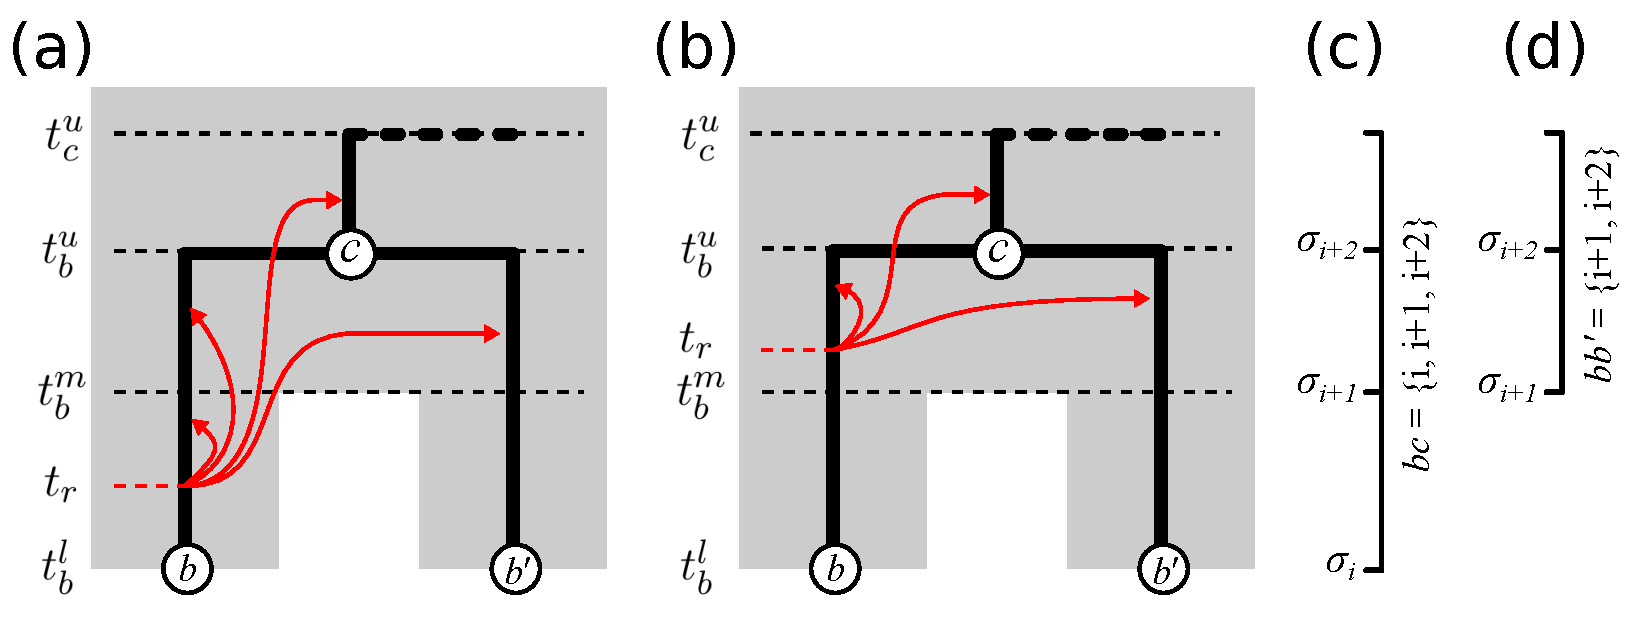
\includegraphics[width=0.75\textwidth]{figures/FigS1-sibling-parent-it2.pdf}
	\caption{
		To calculate the probability that recombination on a genealogy branch
		($b$) leads to a topology change involves summing over the probabilities 
		that a detached lineage does not re-coalesce with either
		itself ($b$), its sibling ($b'$) or its parent ($c$) branches. At the time 
		recombination occurs ($t_r$) the branches $b$ and $b'$ can either exist 
		in different species tree intervals (a) or the same interval (b). This 
		restricts the probability of tree-change outcomes (e.g., shortened coalescent 
		time) until the lowest shared interval between $b$ and $b'$ at time 
		$t_m$. This leads to two ordered sets of intervals (c-d) used in 
		equations 11 and 12.
	}
	\label{fig:fig3}
\end{figure}

% the subsequent two intervals after $t_b^m$, the detached lineage can re-coalesce
% % either with it 
% In this case, we have integrated coalescence probabilities through three sections 
% in which a re-coalescence can produce a category 1, 2, or 3 event: the lower part 
% of branch $b$ when the disconnected branch can reconnect with itself, the upper 
% part of branch $b$ when it can reconnect with either itself or with its sibling,
% and all of branch $c$, with which a coalescent would lengthen branches without 
% changing the topology (Fig.~\ref{fig:fig3}a).

% \begin{equation}
% 	\mathbb{P}(\textrm{topology unchanged} | \mathcal{S},\mathcal{G},b,t_r) = 
% 	\frac{1}{a_i} + \sum_{j=i}^{\mathcal{I}_{b+c}-1}P_{ik}\exp\left\{\frac{a_i}{n_i}t_r\right\} + 
% 	\sum_{j=m}^{\mathcal{I}_b-1}P_{ik}\exp\left\{\frac{a_i}{n_i}t_r\right\}
% \end{equation}

% \begin{equation}
% 	\mathbb{P}(\textrm{topology unchanged} | \mathcal{S},\mathcal{G},b,t_r) = 
% 	\frac{1}{a_i} + \sum_{j=i}^{\mathcal{I}_{bc}-1} 
% 	f(i,j) \exp\left\{\frac{a_i}{n_i}t_r\right\} + 
% 	\sum_{j=m}^{\mathcal{I}_b-1}f(i,j)\exp\left\{\frac{a_i}{n_i}t_r\right\}
% \end{equation}

% \small
\begingroup\makeatletter\def\f@size{9}\check@mathfonts

\begin{equation}
	\mathbb{P}(\textrm{topology-unchanged} | \mathcal{S},\mathcal{G},b,t_r)=
	\begin{dcases}
		\frac{1}{a_i} + 
		\sum_{j=i}^{\mathcal{I}_{bc}-1} f(i,j) \exp\left\{\frac{a_i}{2n_i}t_r\right\} + 
		\sum_{j=m}^{\mathcal{I}_b-1} f(i,j) \exp\left\{\frac{a_i}{2n_i}t_r\right\}, 
		& \text{if } t_r < t_b^m \\
		\\
		2\bigg(
			\frac{1}{a_i} + 
			\sum_{j=i}^{\mathcal{I}_{b}-1} f(i,j)\exp\bigg\{\frac{a_i}{2n_i}t_r\bigg\}
		\bigg) + 
		\sum_{\mathcal{I}_b}^{\mathcal{I}_{bc}-1} f(i,j) \exp\bigg\{
			\frac{a_i}{2n_i}t_r
		\bigg\},
		& \text{if } t_r \ge t_b^m \\
	\end{dcases}
\end{equation}

% \normalsize
\endgroup


% \paragraph{Second case --} Given $t_r$ $>$ $t_b^m$ and 
% $t_r \in [\sigma_i, \sigma_{i+1}] \subset [t_b^m,t_b^u]$ is is necessary

% \noindent In the second case (Fig.~\ref{fig:fig3}b), where $t_r$ $>$ $t_b^m$ and 
% $t_r \in [\sigma_i, \sigma_{i+1}] \subset [t_b^m,t_b^u]$ 
% it is only necessary to integrate over probabilities across a subset of the 
% second section, and across the entire third section described above, from 
% which the following equation can be derived:
% % In this second case $t_r$ occurs after $t_b^m$, such that there are only 
% two distinct sections over which to integrate probabilities of tree changes, 
% corresponding to sections 2 and 3 from the case above (Fig.~\ref{fig:fig3}b).
% In the first section $b$ can re-coalescen with either $b$ or $b'$, 
% is when the detached branch can re-coalesce with itself or its sibling, 
% and the second when it can coalesce with its parent 

% \begin{equation}
% 	\mathbb{P}(\textrm{topology unchanged} | \mathcal{S},\mathcal{G},b,t_r) = 
% 	2\left(\frac{1}{a_i} + \sum_{k=i}^{\mathcal{I}_{b}-1}P_{ik}\exp\left\{\frac{a_i}{n_i}t_r\right\}\right) + 
% 	\sum_{\mathcal{I}_b}^{\mathcal{I}_{b+c}-1}P_{ik}\exp\left\{\frac{a_i}{n_i}t_r\right\}
% \end{equation}

% \begin{equation}
% 	\mathbb{P}(\textrm{topology unchanged} | \mathcal{S},\mathcal{G},b,t_r) = 
% 		2\bigg(
% 			\frac{1}{a_i} + \sum_{j=i}^{\mathcal{I}_{b}-1}f(i,j)\exp\bigg\{
% 				\frac{a_i}{n_i}t_r
% 			\bigg\}
% 		\bigg) + 
% 		\sum_{j=\mathcal{I}_b}^{\mathcal{I}_{bc}-1}f(i,j)\exp\bigg\{
% 			\frac{a_i}{n_i}t_r
% 		\bigg\}
% \end{equation}

\subsubsection{Probability that a recombination event on branch $b$ will not change the topology:}
The probability of a topology-unchanged event occurring on a branch can 
be derived by integrating the previous equation over the entire length of a branch.
% We next present the probability that a recombination event occurring on a focal 
% branch $b$ will not change the tree topology -- i.e., it will result in one of the 
% other two outcomes for which we have derived probabilities: no change or tree change.
% As in Section 2.4, 
 % across the entire length of a branch. 
Here, the terms $p_{b,1}$ and $p_{b,2}$ correspond to components
associated with the two cases described above and in Fig.~\ref{fig:fig3}a-b:
% , the lowest interval...the location of $t_b^m$.}
% through the solution that specifies both a specific branch and time. 

% \begin{equation}
% \begin{aligned}
%     &\mathbb{P}(\textrm{topology unchanged} | \mathcal{S},\mathcal{G},b) = 
%     \frac{1}{t_b^u-t_b^l}\left[\sum_{i=0}^{m-1}p_{b,1}^{(i)}+\sum_{i=m}^{\mathcal{I}_b-1}p_{b,2}^{(i)}\right] \\
%     &where: \\
%     &p_{b,1}^{(i)} = \frac{1}{a_i}\left[d_i+n_i\left(\exp\left\{\frac{a_i}{n_i}\sigma_{i+1}\right\}-\exp\left\{\frac{a_i}{n_i}\sigma_i\right\}\right)\left(\sum_{k=i}^{\mathcal{I}_{b+c}-1}P_{ik}+\sum_{k=m}^{\mathcal{I}_b-1}P_{ik}\right)\right] \\
%     &and: \\
%     &p_{b,2}^{(i)} = \frac{1}{a_i}\left[2d_i + n_i\left(\exp\left\{\frac{a_i}{n_i}\sigma_{i+1}\right\}-\exp\left\{\frac{a_i}{n_i}\sigma_{i}\right\}\right)\left(2\sum_{k=i}^{\mathcal{I}_b-1}P_{ik}+\sum_{k=\mathcal{I}_b}^{\mathcal{I}_{b+c}-1}P_{ik}\right)\right]
%     \end{aligned}
% \end{equation}

\begin{equation}
\begin{aligned}
	&\mathbb{P}(\textrm{topology-unchanged} | \mathcal{S},\mathcal{G},b) = 
	\frac{1}{t_b^u - t_b^l} \Bigg[
		\sum_{i=0}^{m-1}p_{b,1}^{(i)} + 
		\sum_{i=m}^{\mathcal{I}_b-1}p_{b,2}^{(i)}
	\Bigg]
	\\
	&where: 
	\\
	&p_{b,1}^{(i)} = 
		\frac{1}{a_i} \Bigg[
			d_i + 2n_i \bigg(
				\exp\bigg\{\frac{a_i}{2n_i}\sigma_{i+1}\bigg\} - 
				\exp\bigg\{\frac{a_i}{2n_i}\sigma_i\bigg\}
			\bigg)
		\bigg(
			\sum_{j=i}^{\mathcal{I}_{bc}-1}f(i,j) + \sum_{j=m}^{\mathcal{I}_b-1}f(i,j)
		\bigg)
	\Bigg]
	\\
	&and: 
	\\
	&p_{b,2}^{(i)} = 
		\frac{1}{a_i} \Bigg[
			2d_i + 2n_i \bigg(
				\exp\bigg\{\frac{a_i}{2n_i}\sigma_{i+1}\bigg\} - 
				\exp\bigg\{\frac{a_i}{2n_i}\sigma_{i}\bigg\}
			\bigg)
		\bigg(
			2\sum_{j=i}^{\mathcal{I}_b-1}f(i,j) + \sum_{j=\mathcal{I}_b}^{\mathcal{I}_{bc}-1}f(i,j)
		\bigg)
	\Bigg]
    \end{aligned}
\end{equation}

\subsubsection{Probability that a recombination event will not change the topology:}
Finally, by summing the last equation across all branches on a
genealogy we get the probability that a recombination event falling 
uniformly on the genealogy will result in a topology-unchanged event.

\begin{equation*}
    \mathbb{P}(\textrm{topology-unchanged} | \mathcal{S},\mathcal{G}) = 
    \sum_{b \in \mathcal{G}}\frac{t_b^u-t_b^l}{L(\mathcal{G})} 
    \times 
    \mathbb{P}(\textrm{topology-unchanged} | \mathcal{S},\mathcal{G},b)
\end{equation*}

\begin{equation}
    = \frac{1}{L(\mathcal{G})}\sum_{b \in \mathcal{G}}\left[\sum_{i=0}^{m-1}p_{b,1}^{(i)}+\sum_{i=m}^{\mathcal{I}_b-1}p_{b,2}^{(i)}\right]
\end{equation}

\subsubsection{Waiting distance to the next topology change:}

A recombination event either does or does not change the topology
of a genealogy, and therefore, we can of course get the probability
of a topology-change event using our topology-unchanged probability 
statement.
As with the previous waiting distance calculations, the expected distance
until a topology change, given a parameterized MSC model, 
is distributed as an exponential probability density (equation 8). 
Similar to how a rate parameter was derived for the distribution 
of waiting distances until a recombination event (equation 7), 
no-change event (equation 9), or tree-change event (equation 10), 
a rate parameter ($\lambda_t$) can be calculated using equation 13 
to get the probability density for the waiting distance until 
a topology-change event: %, given a genealogy and an MSC model:

\begin{equation}
	\lambda_{t} = 
	L(\mathcal{G}) \times r \times 
	(1 - \mathbb{P}(\text{topology-unchanged} | \mathcal{S},\mathcal{G}))
\end{equation}

% now present the caveats...
This final expectation, however, comes with an important caveat. 
% does come with a caveat. 
Unlike the exact solution for the expected waiting distance to a 
tree-change, the waiting distance for a topology-change is an
approximation, since we have ignored the possible effects of 
intermediate tree-change events that can occur  
during the waiting distance until a topology-change 
% more complicated, % to derive, 
% waiting distance distribution to a \emph{topology} change is more 
% solution for a \emph{topology} change is more complicated, % to derive, 
% due to the possibility of intermediate recombination events 
% because of the possibility of intermediate recombination events 
% that change branch lengths but not the topology 
(e.g., the second and third recombination events in Fig.~\ref{fig:fig2}).
% In other words, during the waiting distance until a topology-change occurs,
% given a specific starting genealogy, the genealogy branch lengths could 
% change, thus affecting the probabilities of subsequent outcomes.
% subsequent recombination events, 
% including the relative probabilities of different categorical types.
% for the next event.
% As these events
% As the branch lengths of intermediate genealogies change this affects the
% rate of subsequent recombination events, and thus 
% These events impact the rate of recombination events and 
% the probability
% that each further recombination event changes
% that such events could change
% the topology of the %newly generated 
% next
% genealogy. 
In other words, the probability of topology-change is not guaranteed to
be homogeneous across some distance of the genome.
This problem similarly arises in a single population model,
where \citet{deng_distribution_2021} have previously
demonstrated that its effect can likely be ignored. We 
re-examine this potential bias with respect to models with 
different levels of population structure, and numbers of samples,
in our validations below.

% This is because the product of $L(\mathcal{G})$ and 
% the probability of a topology-changing recombination event
% does not change significantly 
% (longer genealogies are more likely to experience topology-change).

% Below, we demonstrate the accuracy of our approach, and investigate 
% the potential for biases caused by approximation, by validating our
% results relative to coalescent simulations with recombination.

% For example, when branch lengths become very long the expected 
% waiting distance to the next recombination event becomes very small, 
% and similarly the probability of topology-change decreases. 
% Conversely, if branch lengths are as short as possible within the 
% constraints of a species tree model, waiting distances between 
% events will be longer, and more likely to change the topology, since any 
% new sampled ancestor is more likely to be deeply coalesced. 
% Thus, while lengthening of branch length decreases the probability of 
% topology-change it increases the frequency of overall recombination events, 
% and vice versa, such that tree-change events have little overall effect 
% on the probability of topology-change. 
% Later, we validate 

% by showing that our equations yield accurate 
% waiting distances when compared to coalescent simulations
% even when the ratio of tree to topology changes is high.
% This expectation is investigated below using coalescent simulations.

% , for example, consider the extreme
% case )
% Even as branch lengths increase, reducing the waiting time to the 
% next recombination event, the probability that %the recombination event 
% this event will change the topology decreases. 
% Therefore, we follow their approach by approximating the waiting distance to
% a change in topology using an exponential probability density 
% distribution 
% with the following rate:

%\begin{equation}
%\begin{aligned}
%	&p_r(d|\mathcal{G},\mathcal{S}) = r\beta_\mathcal{S}(\mathcal{G})L(\mathcal{G})\exp\left[-r\beta_\mathcal{S}(\mathcal{G})L(\mathcal{G})d\right]\textrm{,} \\
%	&where \\
%	&\beta_\mathcal{S}(\mathcal{G})=1-\mathbb{P}(\textrm{topology unchanged} | \mathcal{G},\mathcal{S}).
%\end{aligned}
%\end{equation}

\section{Results}
% \label{sec:others}

\subsection{Implementation}
We have implemented our solutions for waiting distance calculations
under the MS-SMC' in the Python package \emph{ipcoal} \citep{mckenzie_ipcoal_2020}.
This includes functions that accept a parameterized MSC model, initial genealogy, 
and recombination rate as input, and return the probabilities of different 
recombination event types. The probabilities can be calculated for specific 
branches and times, for entire branches, or for entire genealogies. 
Functions are also available to calculate the likelihood of observed 
waiting distances between different genealogy changes in an ARG 
using an exponential probability density parameterized by the MS-SMC'.
Below we use the coalescent simulation framework in \emph{ipcoal}, 
based on \emph{msprime} \citep{baumdicker_efficient_2022}
and \emph{toytree} \citep{eaton_toytree_2020}, to 
validate our 
results and investigate the impacts of MSC model parameters.
% models, visualizing results, and validating our equations.
Source code is available at \url{https://github.com/eaton-lab/ipcoal}.
Jupyter notebooks demonstrating the MS-SMC' calculations and with 
reproducible code used for validations in this study are available
at \url{https://github.com/eaton-lab/waiting-distances}.

% tree manipulationpaired with 
% Source code and example jupyter notebooks are available at
% \url{https://github.com/eaton-lab/ipcoal}, including validation against 
% coalescent simulations  software  paired with tree visualizations from
% % Our MS-SMC functions are implemented in the subpackage \emph{ipcoal.smc}. 
% Here we demonstrate
% the accuracy of our solutions relative to simulated tree sequences.
% Source code is available at 
% We adapted our solutions to python code, and we implemented them alongside the phylogenomic simulation package \emph{ipcoal} (an MSC-focused wrapper for the popular population genomic simulator \emph{msprime}) \citep{mckenzie_ipcoal_2020,baumdicker_efficient_2022}. Doing so facilitated three simple, illustrative analyses.

\subsection{Demonstration}
% First, when given a species tree and initial genealogy, we could examine the probability 
Given a parameterized MSC model and initial genealogy the probabilities of 
different types of outcomes of recombination can be calculated and visualized as 
a function of when and where recombination occurs. This is demonstrated on an 
imbalanced 4-tip species tree with \hl{constant} effective population size across 
branches %(see parameters in Table~S2), 
and with a genealogy of seven samples embedded, 
including three from lineage A, two from lineage B, and one from lineages
C and D (Fig.~\ref{fig:fig1}a; see Fig.~\ref{fig:figS-edge-probabilities} for 
detailed parameter settings). 
As a demonstration, the probabilities of no-change, tree-change, and 
topology-change given a recombination event occurring on a branch at a 
particular time (equations 3 and 11, respectively) 
are shown for three selected branches on the example genealogy 
(Fig.~\ref{fig:fig1}b-d). 
Note that the probability of no-change and tree-change events 
are inversely related, and sum to 1, since one or the other must occur as a consequence 
of recombination. By contrast, a topology-change event is a subset of the 
probability of a tree-change; 
% recall that a topology-change event is 
it is a tree-change event where the detached branch re-coalesces with 
a branch other than itself, its sibling, or its parent.

% We then applied our solutions to calculate probabilities of changes given 
% ...Our species tree was proposed arbitrarily with a root height of 1e6 generations and 
% includes branch-specific effective population sizes (Table~S1). 
% Our sampling in the genealogy includes three individuals
% for population A, two individuals for population B, and one individual for each 
% population C and D. The exact parameterization for the model, as well as the 
% code to replicate the analysis, is documented in our supplementary notebooks.
% ...
 % tree model 
% of changes in the genealogy given a recombination event on a specific branch and at a 
% specific time. \textbf{Figure 3} illustrates the selection of three branches from a genealogy 
% embedded in a species tree model. The species tree 
% was unbalanced 
% is imbalanced
% with five tips, 
%had 
% and equal internode distances of 2.5e5 generations, 
% and had 
% with constant Ne of 2e5 across species tree intervals. 
% Parts 

In general, the probability of a no-change event decreases, and the probability
of a tree-change event increases, as recombination occurs closer to the top
end of a branch (further back in time). This makes sense, since when 
recombination occurs at the top of a branch there is less time for it to re-coalesce 
with its same branch. Although this is a general trend, these probabilities do not 
behave monotonically along the length of a branch, as they would in a 
single-population model with constant Ne \citep{deng_distribution_2021}.
Instead, probabilities increase or decrease through the length of each
interval as a function of the probabilities of outcomes in subsequent 
intervals -- which can be higher or lower -- and the probabilities that 
a recombination event causes re-coalescence in those intervals.

For example, consider branch 2, which initially exhibits an increase in the
probability of no-change through its first branch interval from time 0 to
$t_7$, but then a decrease through the next interval from $t_7$ to $W_{AB}$
(Fig.~\ref{fig:fig2}b).
The observed increase through the first interval is influenced by the fact that
a re-coalescence in the subsequent interval is more likely to cause a no-change
event, since that interval contains only two samples instead of three.
% up recombination occurs in this interval the more likely it is to re-coalesce
% in the next interval, where only two instead of three samples are present, such
% that a no-change event is more likely. 
By contrast, within the second interval, as recombination occurs closer to 
the top, it is approaching the next species tree divergence event, where the 
number of samples will increase again, from 2 to 3, 
thus decreasing the probability of a no-change event. In this way, 
the probabilities of different recombination event types represent
an integration over all the positions on a branch where recombination could
occur, and all positions at or above that point, and on the same or different
branches, where a detached branch could reconnect. 

% at any time 
% point incorporates all of the possibilities of re-coalescence at deeper 
% time points.
% while also incorporating potentially variable coalescence rates within 
% different species tree intervals.

Branch 7 provides a clear example for examining the probabilities of 
tree and topology-change events. Of particular interest is the 
interval from $W_{AB}$ to $W_{ABC}$ where these probabilities diverge 
significantly (Fig.~\ref{fig:fig2}c-d). 
% Another example is clear from examining probabilities across branch 7,
% which spans three species tree intervals. 
% To better understand probabilities of tree and topology-change events let 
% us examine branch 7, which spans three species tree intervals. 
% Of particular interest is the large different in probabilities of tree-change versus 
% topology-change from intervals from 
The probability of topology-change decreases faster than the probability of 
tree-change as recombination occurs closer to $t_9$. This is because 
following $t_9$ there is a large stretch of time during which re-coalescence can
only occur with the same branch or its sibling, which can result only in tree-change
events. It is only after $W_{abc}$ that it is once again possible for re-coalescence
to occur with a more distant branch that would result in topology-change. 
If the effective population size of this species tree interval (AB) were greater
then the probability of re-coalescence in a deeper interval would be more likely, 
and the probability of topology-change would decrease less severely near $t_9$. 
This is true more generally as well, as can be seen by comparing edge probabilities
across MSC models with different effective population sizes (Fig.~\ref{fig:figS-edge-probabilities}).
Effective population size affects the rate of re-coalescence, and thus 
has the effect of either smoothing probabilities across intervals when 
N$_e$ is high, or accentuating differences among intervals when N$_e$ is low.

% Fig.~\ref{fig:fig1} panels b, c, and d show the probability that a recombination event 
% falling at each time $t_r$ on the 3 selected genealogy branches results in no change 
% (b), results in a tree change (c), and results in a topology change (d).  
% The tendency of the y-values in (b) to approach 0 and (c) to approach 1 as x-values increase 
% make clear that recombination events falling at the tops of branches 
% (i.e., far right on the x-axis) are increasingly certain to change the branch lengths 
% of the genealogy. This is because any re-coalescence of the detached branch can only occur 
% above the recombination breakpoint. The values in part (d), however, never approach 1 (i.e. 
% certain to produce a topology change). This is because re-coalescence with the parent branch, 
% which would not result in a topology change, is still possible even if 
% a recombination event occurs at the very top of a focal branch. 

%\begin{figure}
%	\centering
	%\fbox{\rule[-.5cm]{4cm}{4cm} \rule[-.5cm]{4cm}{0cm}}
%	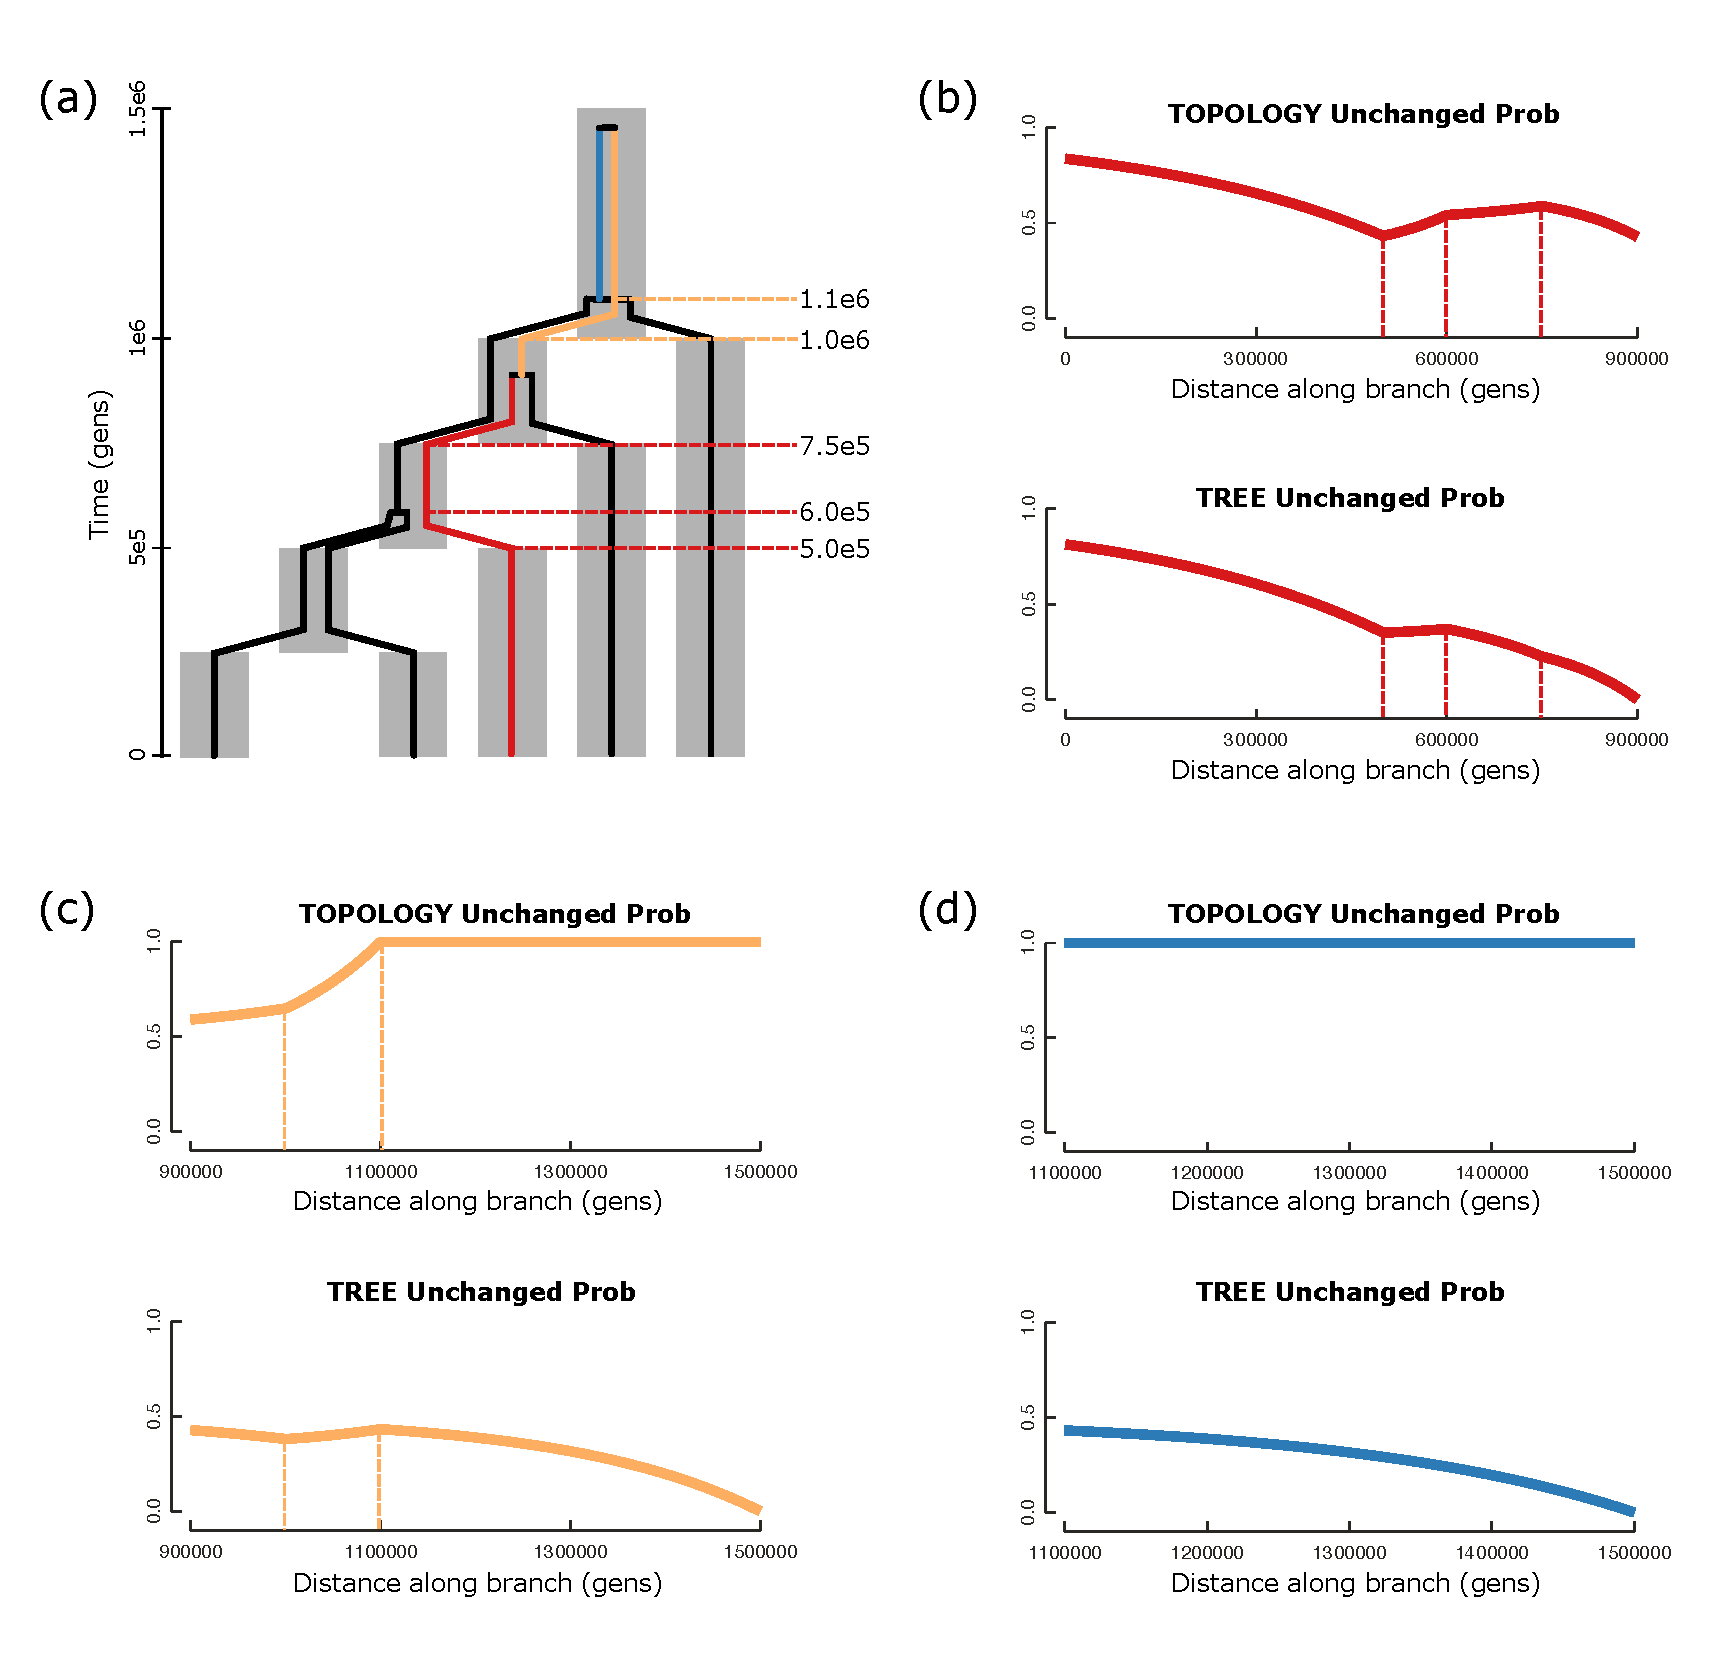
\includegraphics[width=0.9\textwidth]{figures/Fig4-bt_prob.pdf}
%	\caption{Probability that the topology and the tree remain unchanged, given a recombination event at a specific time on a specific branch. The species tree (a) was arbitrarily parameterized as being unbalanced with 5 tips, having internode distances of 2.5e5, and having constant Ne of 2e5. The embedded genealogical tree was randomly generated by \emph{ipcoal} using MSC probabilities. We selected three branches, indicated by three different colors, across which we calculated the probability that the topology would remain unchanged and the tree would remain unchanged if a recombination event were to occur at each time point on the branch (b-d). Dashed lines indicate the beginning and ending times of different intervals on each branch -- that is, either a relevant species tree divergence event or genealogy coalescence event.}
%	 \label{fig:fig3}
%\end{figure}

% This was tested for demographic models with different numbers of lineages;
% different numbers of samples among lineages; 
% and with different MSC model parameters, with the goal of representing scenarios
% spanning from population genetic to deeper-scale phylogenetic datasets. All
% datasets show nearly perfect matching between expected and simulated waiting 
% distances (Fig.~\ref{fig:fig-validation}). 

\subsection{Validation}


\begin{figure}[t]
	\centering
	%\fbox{\rule[-.5cm]{4cm}{4cm} \rule[-.5cm]{4cm}{0cm}}
	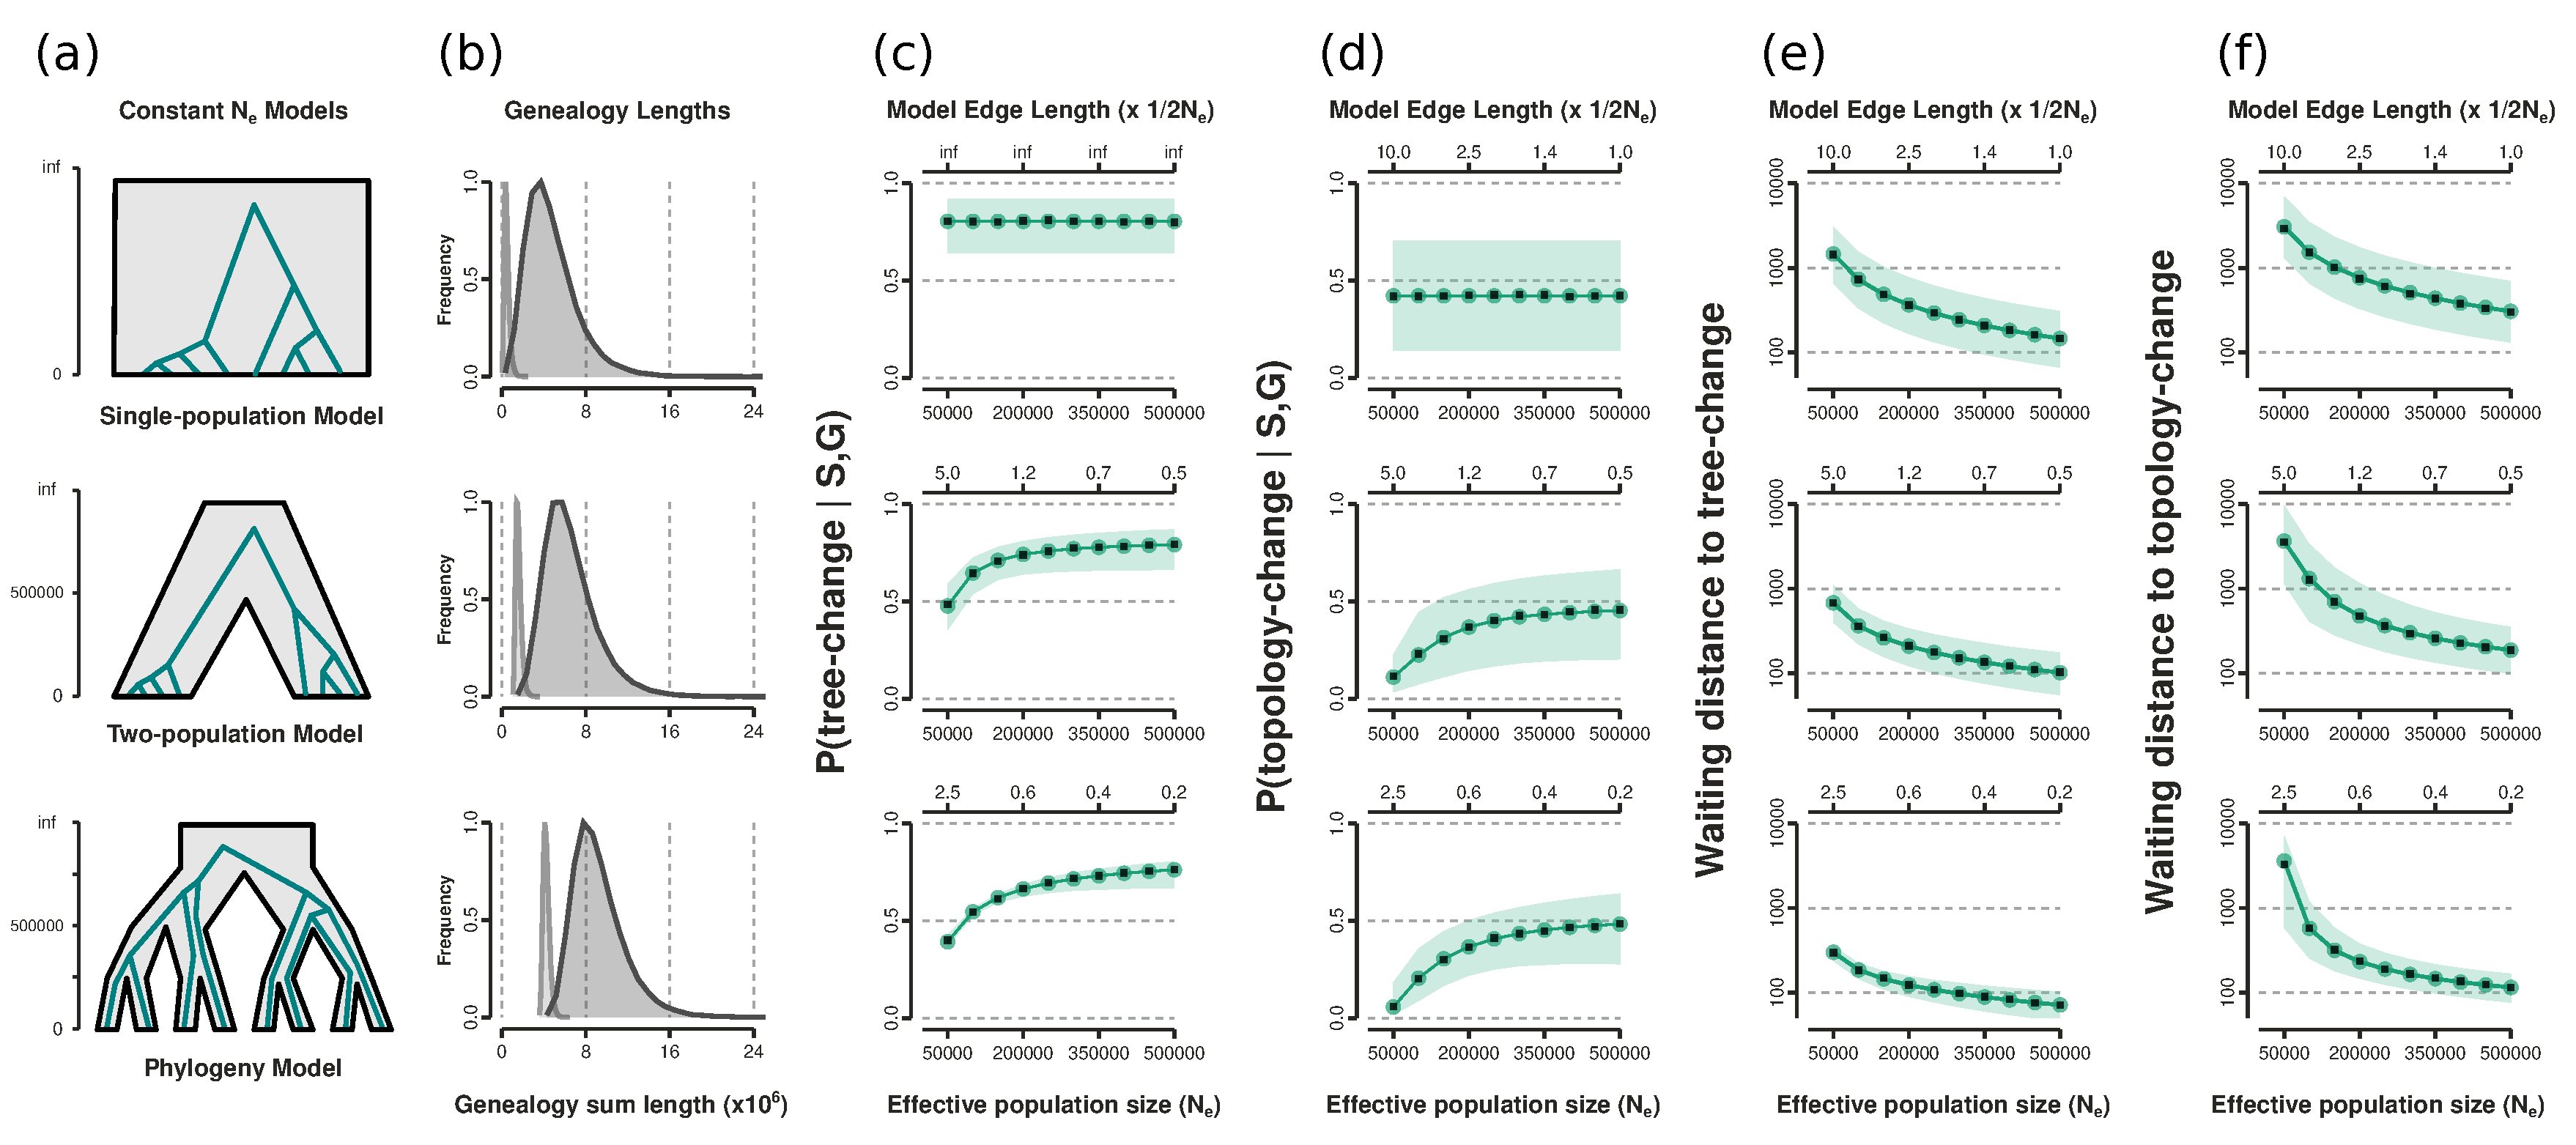
\includegraphics[width=0.99\textwidth]{figures/Fig4-final-validation2.pdf}
	\caption{
		MS-SMC' estimates of waiting distances between recombination
		event types validated against coalescent simulations. Results are 
		shown for three models (a) containing either 1, 2, or 8 populations,
		among which genealogies for 8 samples are embedded. For each model
		10K tree sequences were simulated. 
		(b) The sum of edge lengths across all starting genealogies for each 
		model for the lowest and highest N$_e$ values examined 
		(50K and 500K, respectively).
		(c-d) The mean and 95\% CI (green circle and fill) are shown for analytical
		solutions from the first genealogy in each tree sequence, to be compared 
		with the mean observations across simulated tree sequences (black squares).
		The probabilities of tree-change or topology-change are 
		constant with respect to N$_e$ in a single population model, 
		but vary in models with population structure (also shown with respect to 
		species tree interval lengths in coalescent units, across the top axis). 
		Mean MS-SMC' calculated probabilities match simulated frequencies. 
		(e-f) Waiting distances until tree or topology-change events exhibit 
		less variance in models with population structure. The MS-SMC' calculated 
		waiting distance expectations match very closely to simulated values, 
		but the topology-change waiting distance exhibits slight bias at very low 
		N$_e$ values.
	}
	% Mean expected waiting distances for differently parameterized species tree models. We used four different species trees: two 10-tip trees (a, b), each with 1e6-generation root heights, and two 5-tip trees (c, d) that are subselected from each of the larger trees. For each species tree, we iterated over 9 Ne values ranging from 50000 to 250000, generating 1000 unlinked MSC genealogies at each Ne value and calculating the expected waiting distance to a tree change and to a topology change for each. The mean of the expected waiting distances at each Ne value is presented in the scatterplot accompanying each species tree. Note that the y-axis scale changes from the top row (a, b) to the bottom row (c, d).}
	\label{fig:fig-validation}
\end{figure}


% summary of this sections first goal, and reference to exhaustive supplement figure.
To validate our analytical solutions for the probabilities of different 
recombination event outcomes, and their associated waiting distances, 
we compared our MS-SMC' calculations with coalescent simulations. 
We set up three scenarios with increasing amounts of population structure: 
a single-population model, two-population model, and phylogeny model. 
All analyses used a constant per-site per-generation recombination rate of 
2e-9, and simulated tree sequences using the coalescent with recombination 
(i.e., the "hudson" ancestry model in msprime as opposed to the "smc\_prime" model, 
which is an approximation), unless specified. 
For each model we simulated genealogies for the same total number of samples
(8, unless specified), which were divided evenly among lineages when models 
include multiple populations (Fig.~\ref{fig:fig-validation}a). We examined 
results across a range of parameter settings for a fixed diploid effective 
population size applied to all lineages in a model. 
% When N$_e$ is low, 
% population structure is expected to have large effects, whereas when N$_e$ is 
% high, barriers imposed by population structure are expected to have 
% limited effects.
	
The exponential rate parameter for waiting distances is a product of the 
per-site per-generation recombination rate ($r$), the sum length of edges on the 
current genealogy ($L(\mathcal{G})$), and the probability ($\mathbb{P}$) of the 
specified event type (equations 9, 10, and 14). Across the three models examined,
$r$ remains constant, but both $L(\mathcal{G})$ and $\mathbb{P}$ vary due to 
population structure, where the effect of population structure is scaled by N$_e$. 
Therefore, we examined $L(\mathcal{G})$, $\mathbb{P}$, and the expected waiting 
distance calculated from their product, for each demographic model across a range 
of N$_e$ values (Fig.~\ref{fig:fig-validation}b-f). 
For each value of Ne, 10K tree sequences were simulated. Given the starting tree,
the probability of each event type and expected waiting distances were calculated
under the MS-SMC'. To compare this with the result of a simulated coalescent with
recombination process, we recorded the waiting distance until each recombination
event type first occurred in each tree sequence, and recorded the frequency at which
each event type occurred as the first event in a tree sequence, as a measurement
of its empirical probability.


For each value of Ne, 10K unlinked genealogies were simulated and used as 
starting trees for MS-SMC' calculations of either the expected waiting distance 
until the next tree-change or topology-change event, respectively. 
The mean and 95\% confidence intervals of these MS-SMC' analytical expectations 
align well with mean waiting distances observed in 10K simulated 
tree-sequences, where each tree-sequence contained at least one tree and 
topology-change event.

As expected, waiting distances until tree or topology-change events decrease as
values of Ne increase, and topology-change waiting distances are always larger
than tree-change waiting distances. From a more exhaustive exploration of 
parameter space (Fig.~\ref{supp}) some further generalizations can be made. 
Waiting distance to tree or topology changes tend to be shorter for
larger numbers of samples; more imbalanced species trees; and in species trees with
higher incomplete lineage sorting (shorter internal branch lengths in coalescent
units). 

For a MSC model with relatively shallow divergences, such as a species with 
population structure, it can be valuable to examine the difference in expectations
when the population is modeled as a single population versus multiple structured
populations. For this, we again sampled 10K genealogies across 10 different values
for constant Ne in either a single or two-population MSC model, in which the 
split between the two populations occurred 50K generations ago.
(Fig.~\ref{4b}). 

% what does this mean overall.
It is interesting here to also take note of the scale of waiting distances 
across different MSC model scenarios.
- Previously the expected linkage in phylogenetic datasets could only be computed
through exhaustive simulations (e.g., \citep{McKenzie}). 
- In addition to MSC parameters of divergence times and effective population sizes, 
other factors can also clearly affect the expected distances until ...
Tree shape, tree size, the distribution of samples among species tree 
lineages

% second validation
We also investigated the potential bias present in calculations of 
waiting distances between topology-change events due that may occur
from ignoring tree-change events that occur during the waiting distance
until a topology-change event.
For this, we simulated very long tree-sequences, such that they 
include many topology-change events in which intermediate tree-change 
events arose, but also include many topology-change events that did
not include any intermediate tree-change events. From this, we 
calculate for each type the error between the observed waiting distance
from the starting genealogy until the topology-change event, compared
to the expected waiting distance under the MS-SMC'. We repeated this
for MSC models with different constant effective population sizes which
effectively change the ratio of tree to topology-change events. 

... results are...




\subsection{Investigating bias in topology-change waiting distances}


% with larger Ne values. This occurs for two reasons: first, genealogies with longer 
% branches have a higher probability of any recombination event occurring, since the
% rate is proportional to the sum of edge lengths; second, when Ne is large it is 
% more likely that many genealogy edges will exist in the same species tree intervals
% together, 
% coalescent events are more likely to occur deeper in time


% brief methods description
% Next, we tested the effect of variation in basic species tree parameters on expected waiting 
% distances to tree changes and topology changes (Fig.~\ref{fig:fig3}). We started with four 
% different species trees: two imbalanced and two balanced. For each pair, we used a large tree 
% (10 tips), and a small tree (5 tips) that was pruned from the large tree, with internode 
% distances kept the same. On each species tree, we generated 1000 random \emph{unlinked} 
% genealogies using MSC probabilities and using 
% each of 9 evenly spaced Ne values, ranging from 50000 to 250000. We calculated the expected 
% waiting distance 
% to a tree change and to a topology change for each genealogy/species tree pair, assuming a 
% recombination rate of 1e-9 recombs/bp/generation. In Fig.~\ref{fig:fig3}, we show the mean 
% expected waiting distances to tree and topology changes for each species tree and for each Ne 
% value. The decline in expected waiting distances across Ne values and from small to large 
% trees demonstrates that, on average, waiting distances to tree and topology changes decrease 
% with increasing numbers of tips sampled and with increasing Ne values. 




\subsection{Likelihood framework}
Finally, we demonstrated that a known sequence of genealogies paired with the accompanying
observed waiting distances to next topological change for each can be used to estimate the 
Ne value for species trees with different topologies (Fig.~\ref{fig:fig4}). We used two 
different species trees: one imbalanced, 5-tip tree with internode branches of equal length,
and one 10-tip tree with an irregular topology and branches of variable lengths. Both species 
trees were assigned equal root heights of 1e6 generations and equal Ne values of 150000 on all 
branches, and we simulated a 5e6-bp chromosome for each using \emph{ipcoal}. We broke each 
chromosome down into its component "initial genealogies" -- those that start each segment 
bounded by changes in topology -- and the accompanying segment lengths (i.e. waiting 
distances). Using these values and a known recombination rate of 1e-9 recombs/bp/generation, 
we calculated the likelihood that each of 41 proposed Ne values produced the set of 
genealogies and waiting distances. Using this approach, we recovered a correctly inferred Ne 
value of 150000 for both trees.


\begin{figure}
	\centering
	%\fbox{\rule[-.5cm]{4cm}{4cm} \rule[-.5cm]{4cm}{0cm}}
	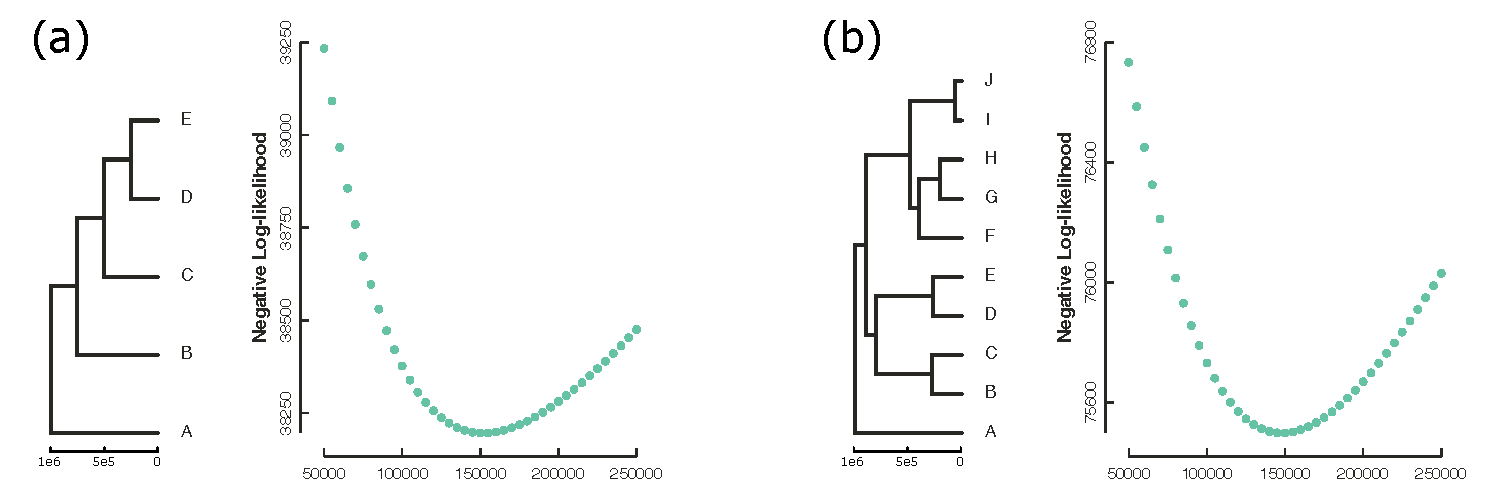
\includegraphics[width=0.9\textwidth]{figures/Fig6-constant_ne_inf.pdf}
	\caption{Inference of species tree Ne values from genealogies, observed waiting distances to topology changes, and recombination rate. We generated two different species trees: Both have root heights of 1e6 generations, but one has five tips, an unbalanced topology, and identical internode lengths, while the other has ten tips, an irregular topology, and irregular branch lengths. Using a recombination rate of 1e-9 recombs/bp/generation and a constant Ne value of 150000 over all branches, we generated a 5MB tree sequence from each species tree using \emph{ipcoal}. Then, we decomposed the alignment into segments bounded by topology changes in the genealogies, and we recorded the initial genealogy for each segment. Finally, we calculated the likelihood of the set of genealogies and waiting distances, along with the recombination rate, at 41 different proposed Ne values. For both sequence alignments, 150000 was correctly inferred as the Ne value.}
	 \label{fig:fig5}
\end{figure}

\section{Conclusions}
% \label{sec:others}

By accounting for the genomic heterogeneity that is expected due to incomplete lineage sorting, the multispecies coalescent model has facilitated the widespread use of multilocus data for phylogenetic inference. As phylogenetic systematics continues to turn toward whole genomes, methods should seek to take advantage of the increased resolution offered by genomic data. The traditional multispecies coalescent model overlooks the process of recombination, assuming that loci represent a single genetic history and that they are completely unlinked. In reality, under a neutral model, species tree parameters and recombination rates will influence the degree of genealogical turnover along a chromosome, potentially resulting in linked loci and/or multiple genealogical topologies per locus. Therefore, not accounting for recombination might mislead analyses. Conversely, incorporating the rates of turnover observed in the data as information could offer further clues for inference of the species tree model that generated it. 

 We began with a simple question: what is the expected turnover rate in topologies along a genome under a species tree model? We generalized a recent solution that used a single population and constant Ne, instead structuring the equations to accept an arbitrary species tree topology and a different, arbitrary Ne value for each species tree branch. These solutions lay a groundwork for exploring how species tree structures affect neutral expectations of genealogical heterogeneity across chromosomes.

%Inference of genealogies along a chromosome is a common goal in population genetics, and similar efforts have been undertaken in phylogenetics. Often, the goal of such efforts is to detect signals of introgression or selection. However, the phylogenetic approaches usually do not explicitly incorporate a model for recombination \citep[e.g.,][]{li2019recombination}. A notable exception to this is ARGweaver-D, which accepts models with population divergence and migration event parameters. Rather than derive probabilities of sequences of genealogical trees, ARGweaver-D uses an MCMC to sample the sequences. This approach is a powerful extension of the single-population ARGweaver method and has been applied successfully to study evolution of hominins, but it is limited to small numbers of samples. Challenges remain for studying properties of tree sequences for larger sets of samples.

Inference of genealogies along a chromosome is a common goal in population genetics, and similar efforts have been undertaken in phylogenetics. Often, the goal of such efforts is to detect signals of introgression or selection. However, the phylogenetic approaches usually do not explicitly incorporate a model for recombination \citep[e.g.,][]{li2019recombination}. Applications of our solutions might provide valuable null hypotheses of genealogical turnover rates by which introgression or selection might be detected. Beyond its use for detecting patterns resulting from non-neutral processes, incorporating recombination in phylogenetic-scale models could also help improve species tree inference. For example, to the extent that they are observable, the empirical distribution of waiting distances to topology changes might be inferred and compared against the expected waiting distances for a proposed species tree model (e.g., \textbf{Figure 5}). Further approaches could determine the distribution of waiting distances to specific types of topology changes, such as those that split up a focal clade.


\subsubsection{Acknowledgements}
This work was supported by the National Science Foundation 
(NSF DEB-2046813 awarded to D.A.R.E. and NSF Graduate Research Fellowship DGE 16-44869 awarded 
to P.F.M.). \hl{Thanks to Yun Deng for guidance on preliminary ideas and to...}


%\subsection{Citations}
%Citations use \verb+natbib+. The documentation may be found at
%\begin{center}
%	\url{http://mirrors.ctan.org/macros/latex/contrib/natbib/natnotes.pdf}
%\end{center}

%Here is an example usage of the two main commands (\verb+citet+ and \verb+citep+): Some people thought a thing \citep{kour2014real, hadash2018estimate} but other people thought something else \citep{kour2014fast}. Many people have speculated that if we knew exactly why \citet{kour2014fast} thought this\dots

%\subsection{Figures}
%\lipsum[10]
%See Figure \ref{fig:fig1}. Here is how you add footnotes. %\footnote{Sample of the first footnote.}
%\lipsum[11]

%\begin{figure}
%	\centering
	%\fbox{\rule[-.5cm]{4cm}{4cm} \rule[-.5cm]{4cm}{0cm}}
%	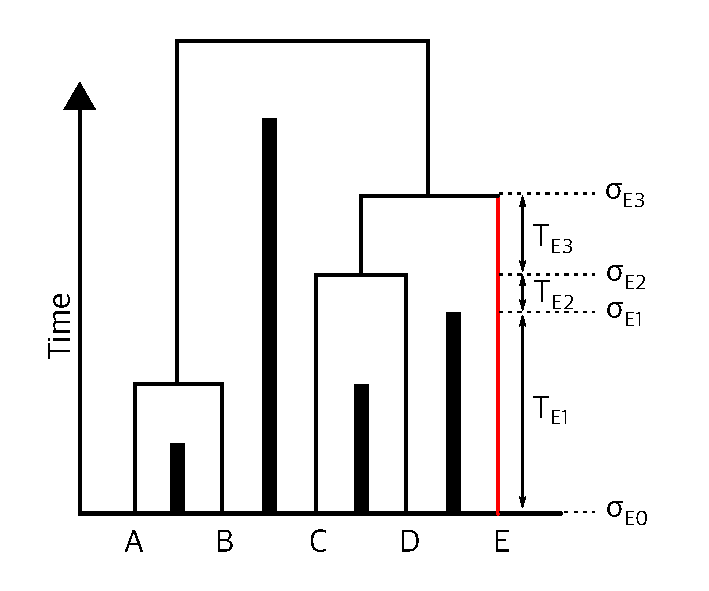
\includegraphics[width=0.6\textwidth]{genealogy_ebranch.pdf}
%	\caption{Sample figure caption.}
%	\label{fig:fig1}
%\end{figure}

%\subsection{Tables}
%See awesome Table~\ref{tab:table}.

%The documentation for \verb+booktabs+ (`Publication quality tables in LaTeX') is available from:
%\begin{center}
%	\url{https://www.ctan.org/pkg/booktabs}
%\end{center}


%\begin{table}
%	\caption{Sample table title}
%	\centering
%	\begin{tabular}{lll}
%		\toprule
%		\multicolumn{2}{c}{Part}                   \\
%		\cmidrule(r){1-2}
%		Name     & Description     & Size ($\mu$m) \\
%		\midrule
%		Dendrite & Input terminal  & $\sim$100     \\
%		Axon     & Output terminal & $\sim$10      \\
%		Soma     & Cell body       & up to $10^6$  \\
%		\bottomrule
%	\end{tabular}
%	\label{tab:table}
%\end{table}

%\subsection{Lists}
%\begin{itemize}
%	\item Lorem ipsum dolor sit amet
%	\item consectetur adipiscing elit.
%	\item Aliquam dignissim blandit est, in dictum tortor gravida eget. In ac rutrum magna.
%\end{itemize}


\bibliographystyle{ecol_let}
\bibliography{references}  

%%% Uncomment this line and comment out the ``thebibliography'' section below to use the external .bib file (using bibtex) .


%%% Uncomment this section and comment out the \bibliography{references} line above to use inline references.
% \begin{thebibliography}{1}

% 	\bibitem{kour2014real}
% 	George Kour and Raid Saabne.
% 	\newblock Real-time segmentation of on-line handwritten arabic script.
% 	\newblock In {\em Frontiers in Handwriting Recognition (ICFHR), 2014 14th
% 			International Conference on}, pages 417--422. IEEE, 2014.

% 	\bibitem{kour2014fast}
% 	George Kour and Raid Saabne.
% 	\newblock Fast classification of handwritten on-line arabic characters.
% 	\newblock In {\em Soft Computing and Pattern Recognition (SoCPaR), 2014 6th
% 			International Conference of}, pages 312--318. IEEE, 2014.

% 	\bibitem{hadash2018estimate}
% 	Guy Hadash, Einat Kermany, Boaz Carmeli, Ofer Lavi, George Kour, and Alon
% 	Jacovi.
% 	\newblock Estimate and replace: A novel approach to integrating deep neural
% 	networks with existing applications.
% 	\newblock {\em arXiv preprint arXiv:1804.09028}, 2018.

%\end{thebibliography}



\section{Supplementary Information}



\beginsupplement

\begin{figure}[p]
	\centering
	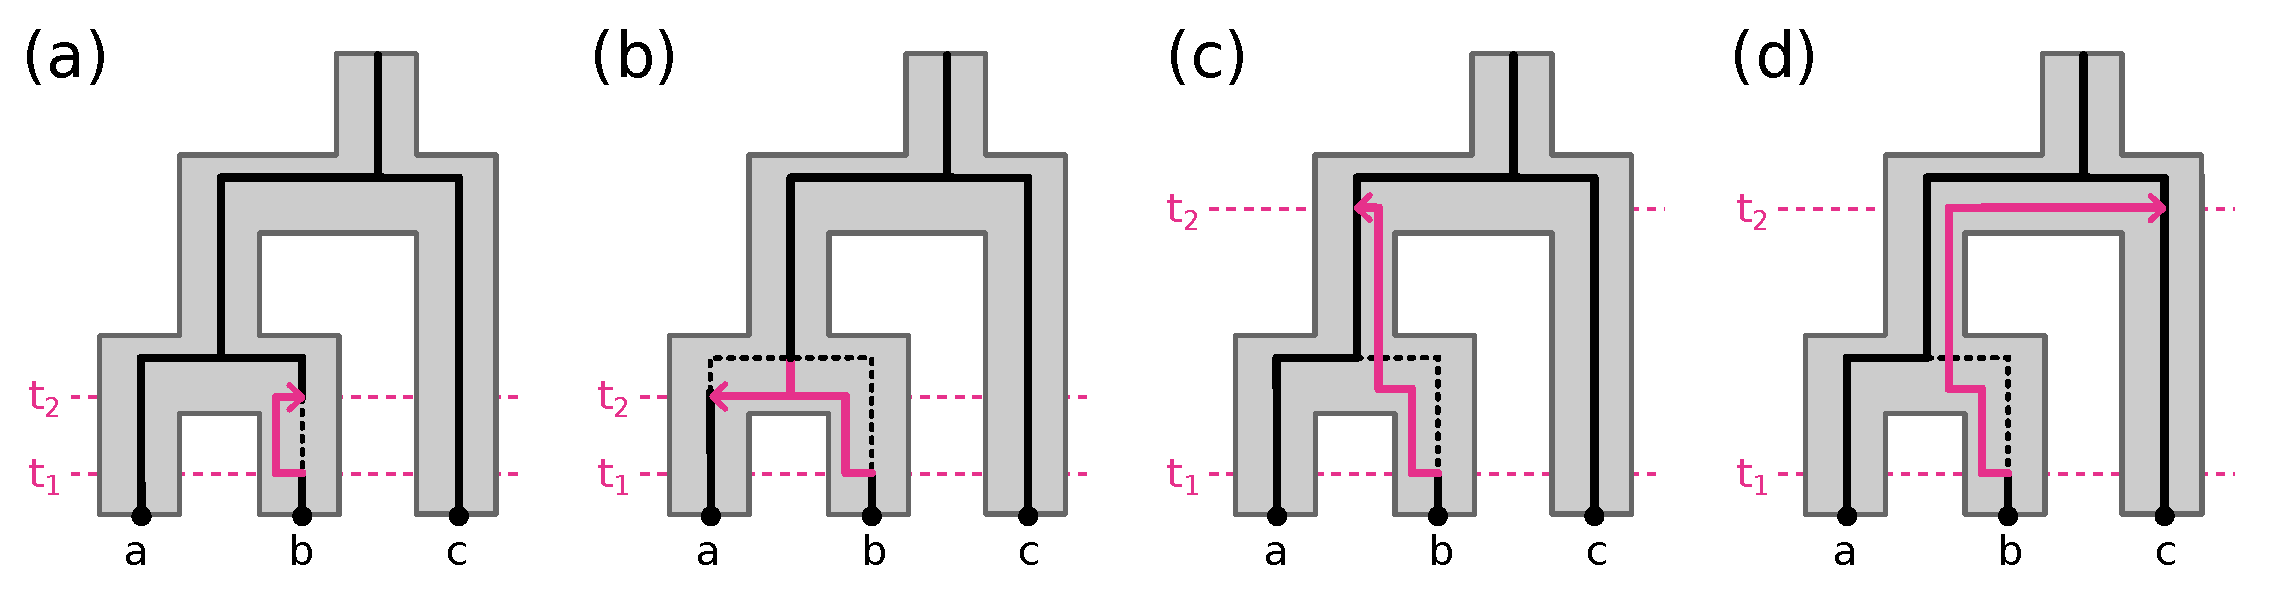
\includegraphics[width=0.9\textwidth]{figures/Fig2-new-recomb-types.pdf}
	\caption{
		Four categories of outcomes of a recombination event occurring on a
		genealogy at time t$_1$, where the detached subtree re-coalesces with
		the remaining lineages under the SMC' process at time t$_2$. (a) The
		detached subtree re-coalesces with the original lineage from which it
		was detached leading to no change between the starting genealogy and 
		subsequent genealogy. (b) The detached subtree re-coalesces with its
		sister lineage prior to their previous coalescence, leading to a shortening
		of their coalescence time. (c) The detached subtree re-coalesces with
		its parent lineage, leading to a lengthening of the coalescent time 
		between the detached subtree lineage and its sister lineage. (d) The
		detached subtree re-coalesces with a lineage other than itself, its sister,
		or its parent lineage, leading to a topology-change. 
	}
     \label{fig:figS-recomb-types}
\end{figure}



\begin{figure}[p]
	\centering
	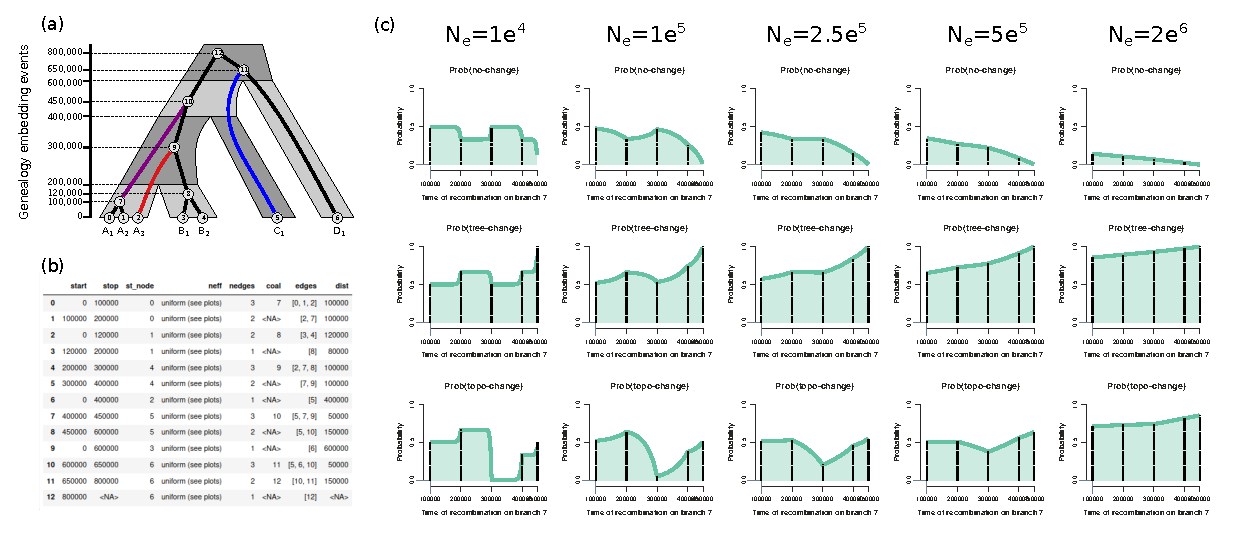
\includegraphics[width=0.9\textwidth]{figures/Fig-S2-edge-probabilities.pdf}
	\caption{
		Probabilities of different recombination event outcomes for a selected 
		genealogy edge as a function of the time at which recombination occurs 
		and a constant effective population size.
		(a) An MSC model with edge lengths in units of generations and an example
		genealogy embedded. (b) An example genealogy embedding table for the MSC
		model and genealogy. (c) Probabilities of different recombination event
		outcomes across genealogy edge 7. When N$_e$ is low probabilities are 
		nearly constant within each interval, since re-coalescent in later intervals
		is unlikely. When N$_e$ is high probabilities change nearly monotonically 
		across the length of an edge, since population structure has little effect
		in constraining the time of re-coalescence.
	}
     \label{fig:figS-edge-probabilities}
\end{figure}



\begin{figure}[p]
	\centering
	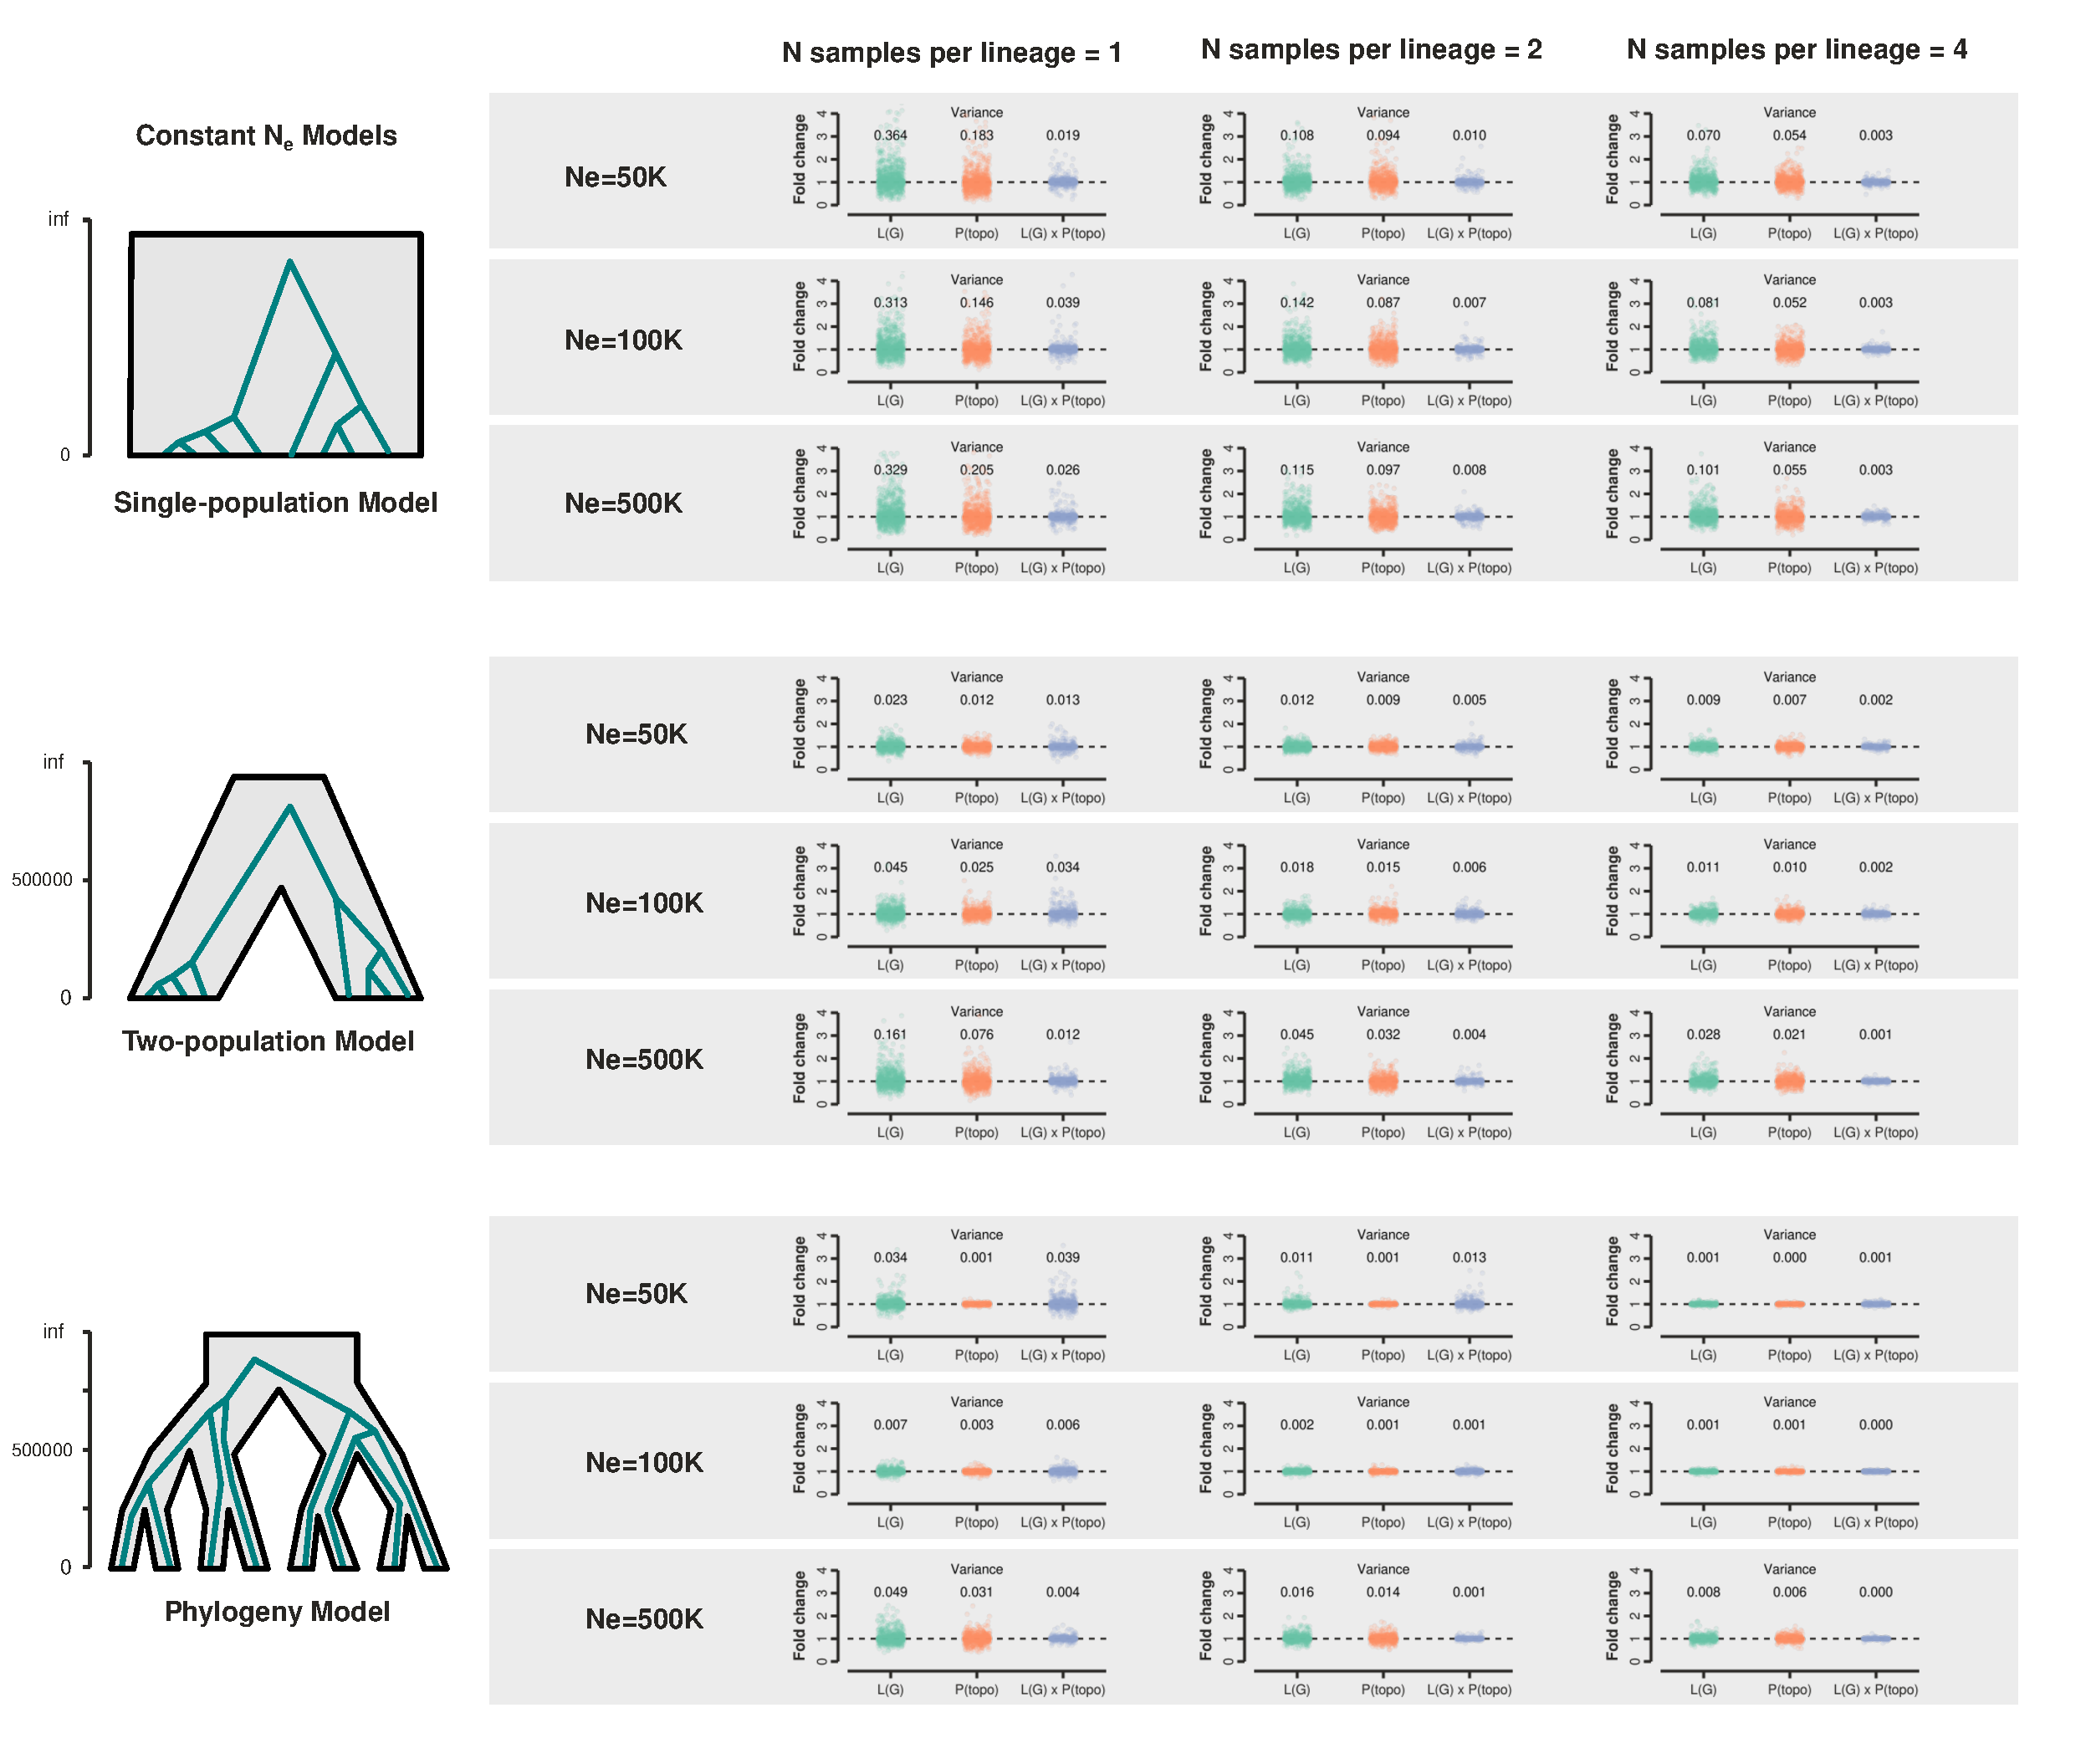
\includegraphics[width=0.9\textwidth]{figures/FigSX-bias.pdf}
	\caption{
		Variance in the fold-change in components affecting the expected waiting 
		distance to a topology change between the starting tree and a subsequent
		tree that has experienced a tree-change event that changed coalescent times
		but not the topology. The sum of genealogical edge lengths (L(G)), the 
		P(topology-change | S,G), and the product of these two terms are shown for
		three different demographic models and with different constant N$_e$ values, 
		and/or numbers of samples per lineage.
		When the fold-change in the product exhibits low variance around 1 the 
		MS-SMC' approximation for the expected waiting distance until a topology-change 
		is expected to be more accurate. Larger effective population sizes and 
		numbers of samples per lineage yield lower variance in the product.
	}
     \label{fig:figS-bias}
\end{figure}


\begin{table}[h]
\centering
\caption{\label{tab:table-S1} 
	A table summarizing the relationships among branches in the genealogical tree embedded in the species tree in Figure 1. 
}
\begin{tabular}[t]{ |c|c|c|c|c|c|c| }
	\toprule
	Branch & $\mathcal{I}_b$ & $t_b^l$ & $t_b^u$ & Parent & Sibling & $t_b^m$ \\
	\midrule
	0  &  1 & 0      & $t_7$  & 7  & 1  & 0          \\
	1  &  1 & 0      & $t_7$  & 7  & 0  & 0          \\
	2  &  3 & 0      & $t_9$  & 9  & 8  & $W_{AB}$   \\
	3  &  1 & 0      & $t_8$  & 8  & 4  & 0          \\
	4  &  1 & 0      & $t_8$  & 8  & 3  & 0          \\
	5  &  4 & 0      & $t_{11}$ & 11 & 6  & $W_{ABCD}$ \\
	6  &  2 & 0      & $t_{11}$ & 11 & 5  & $W_{ABCD}$ \\
	7  &  4 & $t_7$  & $t_{10}$ & 10 & 9  & $t_9$      \\
	8  &  2 & $t_8$  & $t_9$  & 9  & 2  & $W_{AB}$   \\
	9  &  2 & $t_9$  & $t_{10}$ & 10 & 7  & $t_9$      \\
	10 &  3 & $t_{10}$ & $t_{12}$ & 12 & 11 & $t_{11}$     \\
	11 &  1 & $t_{11}$ & $t_{12}$ & 12 & 10 & $t_{11}$     \\
	\bottomrule
\end{tabular}
\end{table}



\newpage
\section{Appendix: Step-by-Step Solution}

Here we describe the derivation of solutions for the MS-SMC' equations in 
greater detail.




\subsection{Notation}

\begin{table}[h]
\centering
\caption{\label{tab:table-S2} 
	Summary of variables used in waiting distance equations. 
}
\begin{tabular}[t]{ |c|l| }
	\toprule
	Variable & Description \\
	\midrule
	$i$          & Integer-valued interval index to which $t_r$ belongs      \\
	$a_x$      & The value of $A(t)$ for all $t_r$ in interval $x$   \\	
	$n_x$          & The value of $N(t_r)$ for all $t_r$ in interval $x$      \\ 
	$\sigma_x$  & The lower boundary, in generations, of interval $x$ \\
	$d_x$      & The length, in generations, of the interval $x$ -- i.e., $\sigma_{x+1} - \sigma_{x}$   \\
	$t_l^b$ & The lower boundary, in generations, of branch $b$  \\
	$t_u^b$ & The upper boundary, in generations, of branch $b$ \\
	$t_m^b$ & The time at which a focal branch $b$ is able to coalesce with its sibling branch \\
	$m$ & Integer-valued interval index whose lower boundary is $t_m^b$ \\
	$\mathcal{I}_b$          & The number of intervals on branch $b$  \\
	$\mathcal{G}$          & The genealogical tree \\
	$\mathcal{S}$   & The species tree with divergence times and branch-specific effective population sizes  \\
	$L(\mathcal{G})$ & The total length of branches in genealogy $\mathcal{G}$ \\
	\bottomrule
\end{tabular}
\end{table}


Assume we have sampled from a species tree $\mathcal{S}$ with $\mathcal{N}$ tips, where 
each tip represents a sampled individual belonging to one of the species. The species tree 
consists of a topology describing the history of population divergences, where each branch 
of the topology has a constant effective diploid population size $N_b$ associated with it. 
Within each branch, coalescence occurs at a constant per-generation rate of $\frac{1}{2N_b}$. 

We begin with a genealogical tree $\mathcal{G}$ sampled from the species tree according 
to coalescent probabilities. This tree is embedded within the species tree so that the 
time of coalescence for any two individuals from different species in $\mathcal{G}$ 
is constrained to occur farther back in time than their species' coalescence times 
in $\mathcal{S}$.

In \citet{deng_distribution_2021}, the genealogical tree was broken into a series of 
intervals so that the number of remaining (not-coalesced) lineages was constant within
each interval. In their method, the number of remaining lineages decreases monotonically
through time from tipward to rootward intervals as lineages coalesce. Our approach is 
similar, except that the intervals are branch-specific and correspond to intervals of 
constant numbers of lineages to coalesce with ($A$) and constant effective population 
size ($N$). Breakpoints may therefore exist where divergences occur in the species 
tree (potentially changing both $A$ and $N$) and where coalescent events occur in 
the genealogical tree (reducing $A$). Unlike in \citet{deng_distribution_2021}, $A$ 
is no longer monotonic, since \emph{species} coalescent events can increase the number
of lineages available for coalescence, while \emph{genealogical} coalescent events
always reduce that number. 

The intervals within each branch of $\mathcal{T}$ are each assigned an index increasing
from $0$ to $\mathcal{I}_b-1$, where $\mathcal{I}_b$ is the total number of intervals
in the branch. The times in generations marking the lower and upper bounds of each 
branch $b$ are notated $t_l^b$ and $t_u^b$, respectively. Each interval of index $x$
is bounded by times $\sigma_x$ and $\sigma_{x+1}$.

% \subsection{The distribution of distances to any change in a genealogical tree}
% Our goal is to derive a distribution of waiting distances to the next tree change
% given a species tree and current genealogy.
We begin with a genealogical tree $\mathcal{G}$ sampled from the species tree according to coalescent probabilities. This tree is embedded within the species tree so that the time of coalescence for any two individuals from different species in $\mathcal{G}$ is constrained to occur farther back in time than their species' coalescence times in $\mathcal{S}$.

\subsubsection{Given a branch and a time}
We begin by assuming a specific branch and time of a recombination event. We then 
integrate across possible times on that branch, and we sum across all branches on
the tree to solve for the probability of the genealogy being unchanged given any 
recombination event. Finally, we incorporate this probability into the exponential
distribution presented in Equation 4.

% \begin{equation}
% 	\mathbb{P}(\textrm{tree unchanged} | b,t,\mathcal{T},\mathcal{S}) = 
% 	\int_{t}^{t^u_b}\frac{1}{A(\tau)}p(\tau|t)d\tau
% \end{equation}
The intervals within each branch of $\mathcal{G}$ are each assigned an index increasing from $0$ to $\mathcal{I}_b-1$, where $\mathcal{I}_b$ is 
the total number of intervals in the branch. The times in generations marking the lower and upper bounds of each branch $b$ are notated $t_l^b$ and $t_u^b$, 
respectively. Each interval of index $x$ is bounded by times $\sigma_x$ and $\sigma_{x+1}$.

Where $A(\tau)$ is the number of lineages able to be coalesced with at any time $\tau$, 
and $p(\tau|t_r)$ is the exponential probability density of coalescing any time 
after the recombination event. Thus, we are integrating over the probability
of coalescence along the path of species tree intervals traversed
by branch $b$, starting at the time of recombination and ending at the 
end of the branch. If the branch spans only a single genealogy embedding 
interval then $A(\tau)$ and $N(\tau)$

\hl{Fixing this section is required...}

Through this series of one or more genealogy embedding intervals the 

up to that time through the species tree intervals that are traversed
by branch $b$, which can involve changing numbers of samples over time (A(t)), 
and changing effective population sizes (N(t)).
Here we define the coalescence rate at time $\tau$ as $\frac{A(\tau)}{N(\tau)}$. 
Note that this differs from \citet{deng_distribution_2021}, 
since our branch lengths are in units of generations rather than in
coalescent units. 

% who defined the 
% coalescent rate over an interval using the more common compound 
% metric of coalescent time units (time in generations /2N). 
% For the purposes of our equations it is simpler to  better to define define time in generations from the
% coalescent probability at any unit of time. per unit
% time, 

\begin{equation}
	\mathbb{P}(\textrm{tree unchanged} | b,t,\mathcal{G},\mathcal{S}) = \int_{t}^{t^u_b}\frac{1}{A(\tau)}p(\tau|t)d\tau
\end{equation}

% coalescence rate.

\begin{equation}
	= \int_{t}^{t^u_b}\frac{1}{A(\tau)} \frac{A(\tau)}{N(\tau)}
	e^{-\int_t^\tau{}\frac{A(s)}{N(s)}ds} d\tau
\end{equation}


\begin{equation}
	= \int_{t}^{t^u_b}\frac{1}{N(\tau)}e^{-\int_t^\tau{}\frac{A(s)}{N(s)}ds} d\tau
\end{equation}



We can now take advantage of the fact that the rate of coalescence is piecewise-constant. We split the equation into one interval $i$ whose length depends on $t$ (it ranges from $t$ until the upper limit of its interval, $\sigma_{i+1}$) and we add to it integrals across intervals that are above it on the same branch, which are predefined by their upper and lower $\sigma$ values:

\begin{equation}
	= \int_{t}^{\sigma_{i+1}} \frac{1}{N(\tau)}\exp\left(-\int_{t}^{\tau}\frac{A(s)}{N(s)}ds\right)d\tau + \sum_{k=i+1}^{\mathcal{I}_b-1}\int_{\sigma_{k}}^{\sigma{k+1}}\frac{1}{N(\tau)}\exp\left(-\int_{t}^{\tau}\frac{A(s)}{N(s)}ds\right)d\tau
\end{equation}

We solve first term and later terms separately:

\paragraph{First term --}

\begin{equation}
	= \frac{1}{a_i} - \frac{1}{a_i}e^{-\frac{a_i}{n_i}\sigma_{i+1}}e^{\frac{a_i}{n_i}t}
\end{equation}

\begin{equation}
	= \frac{1}{a_i} +P_{ii}e^{\frac{a_i}{n_i}t}
\end{equation}

\paragraph{Later terms --}

\begin{equation}
	= \sum_{k=i+1}^{\mathcal{I}_b-1} e^{\frac{a_i}{n_i}t} \exp\left(-\frac{a_i}{n_i}\sigma_{i+1}-\sum_{q=i+1}^{k-1} \frac{a_q}{n_q}T_q\right)\left(\frac{1}{a_{k}}(1-e^{-\frac{a_{k}}{n_{k}}T_{k}})\right)
\end{equation}

\begin{equation}
	= \sum_{k=i+1}^{\mathcal{I}_b-1} e^{\frac{a_i}{n_i}t} P_{ik}
\end{equation}

Adding these together, we are left with the solution:

\begin{equation}
	\mathbb{P}(\textrm{tree unchanged} | b,t,\mathcal{G},\mathcal{S}) = \frac{1}{a_i}+\sum_{k=i}^{\mathcal{I}_b-1}{P_{ik}e^{\frac{a_i}{n_i}t}}
\end{equation}

\subsubsection{Across a full branch}

Having solved for the probability of the genealogical tree being unchanged given the time $t$ of the recombination event, our next step is to integrate this equation across the branch with respect to $t$:

\begin{equation}
	\mathbb{P}(\textrm{tree unchanged} | b,\mathcal{G},\mathcal{S}) = \frac{1}{t^u_b-t^l_b} \int_{t_b^l}^{t_b^u} \mathbb{P}(\textrm{tree unchanged} | b,t,\mathcal{G},\mathcal{S})dt
\end{equation}

Plugging in Equation 17 above, we find:

\begin{equation}
	= \frac{1}{t^u_b-t^l_b}\sum_{i=0}^{\mathcal{I}_b-1}\frac{1}{a_i}d_i + \left(e^{\frac{a_i}{n_i}\sigma_{i+1}}-e^{\frac{a_i}{n_i}\sigma_i}\right)\left[-\frac{n_i}{a_i^2}e^{-\frac{a_i}{n_i}\sigma_{i+1}} + \frac{n_i}{a_i}\left(\sum_{k=i+1}^{\mathcal{I}_b-1}\exp\left(-\frac{a_i}{n_i}\sigma_{i+1}-\sum_{q = i+1}^{k-1}\frac{a_q}{n_q}T_q\right)\frac{1-\exp(-\frac{a_{k}}{n_{k}}T_{k})}{a_{k}}\right)\right]
\end{equation}

\subsubsection{Across the whole tree}

At last, we can calculate the probability that, given a recombination event, the genealogical tree is unchanged. We do this by weighting each branch by its proportion of the total tree length and summing across the unchanging probabilities for all branches:

\begin{equation}
	\mathbb{P}(\textrm{tree unchanged} | \mathcal{G},\mathcal{S}) = \sum_{b=1}^{2N-2}\left[\frac{t^u_b-t^l_b}{L(\mathcal{G})}\right]\mathbb{P}(\textrm{tree unchanged} | b,\mathcal{G},\mathcal{S})
\end{equation}

To derive the waiting distance to the next tree change, we incorporate the value of $1-\mathbb{P}(\textrm{tree unchanged} | \mathcal{G},\mathcal{S})$ into the exponential distribution describing the waiting distance to the next recombination event (introduced in Equation 4):
\begin{equation}
\begin{aligned}
	&p_r(d|\mathcal{G},\mathcal{S}) = r\alpha_\mathcal{S}(\mathcal{G})L(\mathcal{G})\exp\left[-r\alpha_\mathcal{S}(\mathcal{G})L(\mathcal{G})d\right]\textrm{,} \\
	&where \\
	&\alpha_\mathcal{S}(\mathcal{G})=1-\mathbb{P}(\textrm{tree unchanged} | \mathcal{G},\mathcal{S}).
\end{aligned}
\end{equation}

\subsection{The distribution of distances to a change in genealogical topology}

Next, we attempt to further exclude recombination events. We filter out recombination events of categories 2 and 3, which just change branch lengths, to isolate the probability that a recombination event changes the \emph{topology} of the tree.

As in the first section, we treat branches individually and then sum across them. However, we have to designate new variables. We now consider two lineages in addition to the focal lineage $b$: the lineage $b'$ that $b$ coalesces with, and the lineage $c$ that is ancestral to $b$ and $b'$. We also designate the timepoint $t_b^m$, which we use to break the problem into two cases. While the single-population example in \citet{deng_distribution_2021} uses $t_{b'}^l$ as this breakpoint, the species tree introduces more complexity, and we instead use the maximum of three values: $t_{b'}^l$, $t_{b}^l$, and $t_{(b,b')}^w$, which we define as the merging time for the species tree branches separating $b$ and $b'$ (Figure 6).

\begin{figure}
	\centering
	%\fbox{\rule[-.5cm]{4cm}{4cm} \rule[-.5cm]{4cm}{0cm}}
	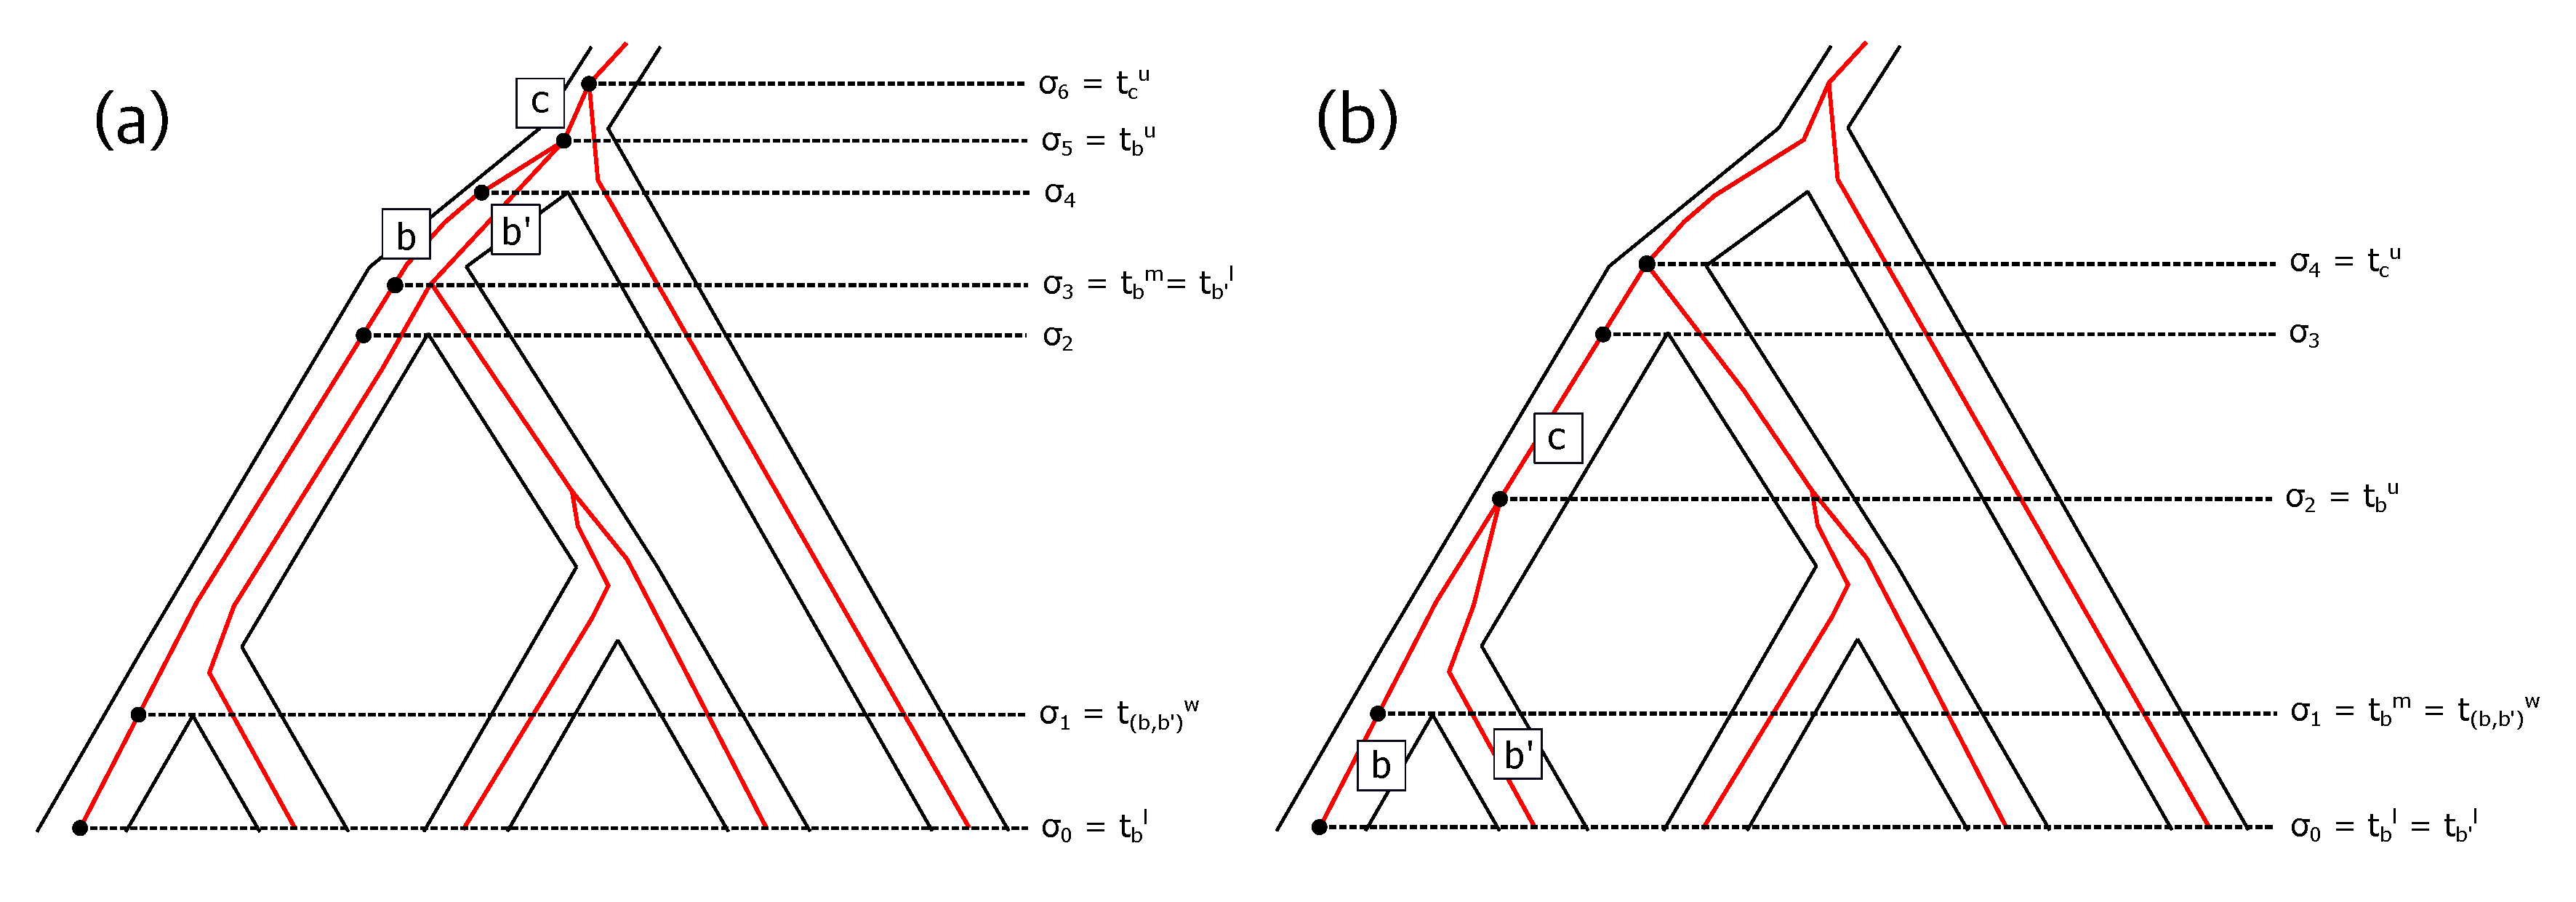
\includegraphics[width=0.9\textwidth]{figures/FigS1-topology_illustration.pdf}
	\caption{Illustrating the parameters for calculating the distribution of distances to a change in the topology of a genealogy. Panels (a) and (b) show slightly different genealogies embedded in the same species tree. In both (a) and (b), the focal branch $b$ is the one leading from the left-most species. Branches $c$ and $b'$ -- the parent and sibling branches, respectively -- are also both labeled. Note that in (a), $t_b^m$ corresponds to $\sigma_3$, while in (b) it corresponds to $\sigma_1$.}
	% \label{fig:fig5}
\end{figure}

\begin{equation}
	\mathbb{P}(\textrm{topology unchanged} | b,\mathcal{G},\mathcal{S}) = \frac{1}{t_b^u-t_b^l}\int_{t_b^l}^{t_b^u}\mathbb{P}(\textrm{topology unchanged} | b,t,\mathcal{G},\mathcal{S})dt
\end{equation}

\begin{equation}
	= \frac{1}{t_b^u-t_b^l}\left[\left(\int_{t_b^l}^{t_b^m}+\int_{t_b^m}^{t_b^u}\right)\mathbb{P}(\textrm{topology unchanged} | b,t,\mathcal{G},\mathcal{S})dt\right]
\end{equation}

Where $t^m_b=\max\{t^w_{(b,b')},t_{b'}^l,t_b^l\}$.

\subsubsection{Given a branch and a time}

As in \citet{deng_distribution_2021}, we break the problem into two cases: a first case in which $t$ belongs to the interval from the base of the focal branch to $t^m_b$, and a second case in which $t$ belongs to the interval from $t^m_b$ to $t^u_b$. 

\paragraph{First case --} Given $t \in [\sigma_i, \sigma_{i+1}] \subset [t_b^l,t_{b}^m]$:

\begin{equation*}
	\mathbb{P}(\textrm{topology unchanged} | b,t,\mathcal{G},\mathcal{S}) = \int_{t}^{t_b^m}\frac{1}{A(\tau)}\rho(\tau|t)d\tau + \int_{t_b^m}^{t_b^u}\frac{2}{A(\tau)}\rho(\tau|t)d\tau + \int_{t_b^u}^{t_c^u}\frac{1}{A(\tau)}\rho(\tau|t)d\tau
\end{equation*}

\begin{equation}
	= \frac{1}{a_i} + \sum_{k=i}^{\mathcal{I}_{b+c}-1}P_{ik}e^{\frac{a_i}{n_i}t} + \sum_{k=m}^{\mathcal{I}_b-1}P_{ik}e^{\frac{a_i}{n_i}t}
\end{equation}

The second case is solved in a similar manner, although we eliminate the first integral:

\paragraph{Second case --} Given $t \in [\sigma_i, \sigma_{i+1}] \subset [t_b^m,t_b^u]$:

\begin{equation*}
	\mathbb{P}(\textrm{topology unchanged} | b,t,\mathcal{G},\mathcal{S}) = \int_{t}^{t_b^u}\frac{2}{A(\tau)}\rho(\tau|t)d\tau + \int_{t_b^u}^{t_c^u}\frac{1}{A(\tau)}\rho(\tau|t)d\tau
\end{equation*}

\begin{equation}
	= 2\left(\frac{1}{a_i} + \sum_{k=i}^{\mathcal{I}_{b}-1}P_{ik}e^{\frac{a_i}{n_i}t}\right) + \sum_{\mathcal{I}_b}^{\mathcal{I}_{b+c}-1}P_{ik}e^{\frac{a_i}{n_i}t}
\end{equation}

\subsubsection{Across a full branch}

Now we derive the overall probability that a recombination event falling on a specific branch will change the topology. We integrate across values of $t$ and sum the two cases defined above, while assuming a uniform probability of the recombination event occurring at any time along the branch:

\paragraph{First case --}

\begin{equation}
	\int_{t_b^l}^{t_b^m}{\mathbb{P}(\textrm{topology unchanged} | b,t,\mathcal{G},\mathcal{S})}=\sum_{i=0}^{m-1}\frac{1}{a_i}\left[d_i+n_i\left(\exp\left(\frac{a_i}{n_i}\sigma_{i+1}\right)-\exp\left(\frac{a_i}{n_i}\sigma_i\right)\right)\left(\sum_{k=i}^{\mathcal{I}_{b+c}-1}P_{ik}+\sum_{k=m}^{\mathcal{I}_b-1}P_{ik}\right)\right]
\end{equation}

\paragraph{Second case --}

\begin{equation}
	\int_{t_b^m}^{t_b^u}{\mathbb{P}(\textrm{topology unchanged} | b,t,\mathcal{G},\mathcal{S})}=\sum_{i=m}^{\mathcal{I}_b-1}\frac{1}{a_i}\left[2d_i + n_i\left(\exp\left(\frac{a_i}{n_i}\sigma_{i+1}\right)-\exp\left(\frac{a_i}{n_i}\sigma_i\right)\right)\left(2\sum_{k=i}^{\mathcal{I}_b-1}P_{ik}+\sum_{k=\mathcal{I}_b}^{\mathcal{I}_{b+c}-1}P_{ik}\right)\right]
\end{equation}

\paragraph{Result --}
\begin{equation}
    \mathbb{P}(\textrm{topology unchanged}|b, \mathcal{G},\mathcal{S}) = \frac{1}{t_b^u-t_b^l}\left[\sum_{i=0}^{m-1}p_{b,1}^{(i)}+\sum_{i=m}^{\mathcal{I}_b-1}p_{b,2}^{(i)}\right]
\end{equation}

\subsubsection{Across the whole tree}

Finally, we sum across all branches to find the probability of a recombination event changing the topology of the tree:

\begin{equation*}
    \mathbb{P}(\textrm{topology unchanged}| \mathcal{G},\mathcal{S}) = \sum_{b \in \mathcal{G}}\frac{t_b^u-t_b^l}{L(\mathcal{G})} \times \mathbb{P}(\textrm{topology unchanged}|b, \mathcal{G},\mathcal{S})
\end{equation*}

\begin{equation}
    = \frac{1}{L(\mathcal{G})}\sum_{b \in \mathcal{G}}\left[\sum_{i=0}^{m-1}p_{b,1}^{(i)}+\sum_{i=m}^{\mathcal{I}_b-1}p_{b,2}^{(i)}\right]
\end{equation}






\end{document}
